\documentclass[9pt,pdf,utf8,hyperref={unicode},aspectratio=169]{beamer}

%Привычный шрифт для математических формул
\usefonttheme[onlymath]{serif}
\mode<presentation>
{
    \usetheme{boxes}
    \beamertemplatenavigationsymbolsempty

    \setbeamercovered{transparent}
    \setbeamertemplate{navigation symbols}{}
    
    \setbeamertemplate{footline}[frame number]
    \setbeamertemplate{caption}[numbered]
    % \setbeamersize{text margin left=0.5em, text margin right=0.5em}
}

% Дополнительные библиотеки
\usepackage[T2A]{fontenc}
\usepackage[english, russian]{babel}
\usepackage[utf8]{inputenc}
\usepackage{amsmath,amssymb}
\usepackage{indentfirst}
\usepackage{changepage}
\usepackage{enumerate}
\usepackage{mathtools}
\usepackage{multicol}
\usepackage{multirow}
\usepackage{ragged2e}
\usepackage{multicol}
\usepackage{diagbox}
\usepackage{wrapfig}
\usepackage{comment}
\usepackage{subfig}
\usepackage{array}
\usepackage{color}
\usepackage{tikz}
\usepackage{url}
\usepackage{bm}

\usetikzlibrary{trees}

% Определение дополнительных функций
\DeclareMathOperator*{\plim}{\mathop{plim}}
\DeclareMathOperator{\prob}{\mathbf{P}\!}
\DeclareMathOperator{\arctanh}{arctanh}
\DeclareMathOperator{\mmode}{mode}
\DeclareMathOperator{\rank}{rank}
\DeclareMathOperator{\diag}{diag}
\DeclareMathOperator{\sign}{sign}
\DeclareMathOperator{\cov}{cov}
\DeclareMathOperator{\pow}{pow}
\DeclareMathOperator{\med}{med}

\def\argmin#1{ \mathop{\text{argmin}}\limits_{#1} }
\def\argmax#1{ \mathop{\text{argmax}}\limits_{#1} }

\renewcommand{\leq}{\leqslant}
\renewcommand{\geq}{\geqslant}

\DeclareMathOperator{\FWER}{FWER}
\DeclareMathOperator{\FDR}{FDR}
\newtheorem{Th}{Теорема}
\newtheorem{Def}{Определение}

% Основная часть


\title[Регрессионный анализ]{Прикладной статистический анализ данных\\ Регрессионный анализ}
\author{Андрей Грабовой}
\date{}

\begin{document}
\tikzstyle{every node}=[draw=black,thick,anchor=west]
\tikzstyle{selected}=[draw=red,fill=red!30]
\tikzstyle{optional}=[dashed,fill=gray!50]

\begin{frame}
    \titlepage
\end{frame}

\section{Построение и свойства}
\subsection{Введение}


\begin{frame}{Первое появление}
%%%%%%%%%%%%%%%%%%%%%%%%%%%%%%%%%%%%%%%%%%%%%%%%%%%%%%%%%%%%%%%%%%%%%%%
% Впервые термин регрессия появился в конце XIX века в работе Френсиса Гальтона. В этой работе «Регрессия к середине в наследственности роста» Френсис Гальтон исследовал зависимость между средним ростом детей и средним ростом их родителей и обнаружил, что отклонение роста детей от среднего составляет примерно 2/3 отклонения роста родителей от среднего. Казалось бы, со временем люди должны рождаться все ближе и ближе к среднему росту. На самом деле, естественно, этого не происходит. Лучше понять эффект регрессии к среднему позволяет другое творение Френсиса Гальтона, которое называется машина, или доска, Гальтона.
% Это механическая машина, в которой сверху в центральной части нахо- дятся шарики. Когда открывается заслонка, шарики начинают постепенно сыпаться вниз, ударяясь о штырьки, которые расположены на одинаковом расстоянии друг от друга. При каждом соударении шарика со штырьком вероятности того, что он упадет налево и направо от штырька, равны. Посте- пенно шарики начинают собираться в секциях внизу в гауссиану, или плот- ность нормального распределения.
% Чтобы понять эффект регрессии к среднему, давайте мысленно подставим к машине Гальтона снизу еще одну такую же машину. Если теперь убрать перегородку, которая удерживает шарики в верхней половине, они начнут постепенно осыпаться вниз и сформируют внизу еще одну такую же гауссиану. Если зафиксировать какой-то конкретный шарик в нижней половине ближе к краю, то откажется, что с достаточно большой вероятностью этот шарик пришел не из ячейки, которая находится в верхней половине прямо над ячейкой, в которой он оказался внизу, а от ячейки ближе к середине. Это происходит просто потому, что в середине шариков больше.
% Эффект регрессии к среднему проявляется во многих практических задачах. Например, если дать студентам очень сложный тест, большую роль в том, насколько хорошо они его пройдут, будут играть не только их знания по предмету, но и везение, то есть случайный фактор. Поэтому, если изолировать 10% студентов, которые прошли тест лучше всех (набрали больше всего баллов) и дать им еще один вариант теста, то средний балл в этой группе скорее всего упадет. Просто потому что люди, которым повезло в первый раз, скорее всего уже не будут так удачливы во второй — в этом и состоит эффект регрессии к середине.
% Френсис Гальтон был основоположником дактилоскопии, исследовал явление синестезии, внес существенный вклад в метеорологию, впервые описав циклоны и антициклоны, а также, например, изобрел ультра- звуковой свисток для собак. Но именно регрессия и по сей день остается одним из наиболее важнейших инструментов, к которому он приложил руку.
%%%%%%%%%%%%%%%%%%%%%%%%%%%%%%%%%%%%%%%%%%%%%%%%%%%%%%%%%%%%%%%%%%%%%%%
    Впервые такая постановка появляется в работе Гальтона 1885~г. <<Регрессия к середине в наследственности роста>>.

    \begin{center}
            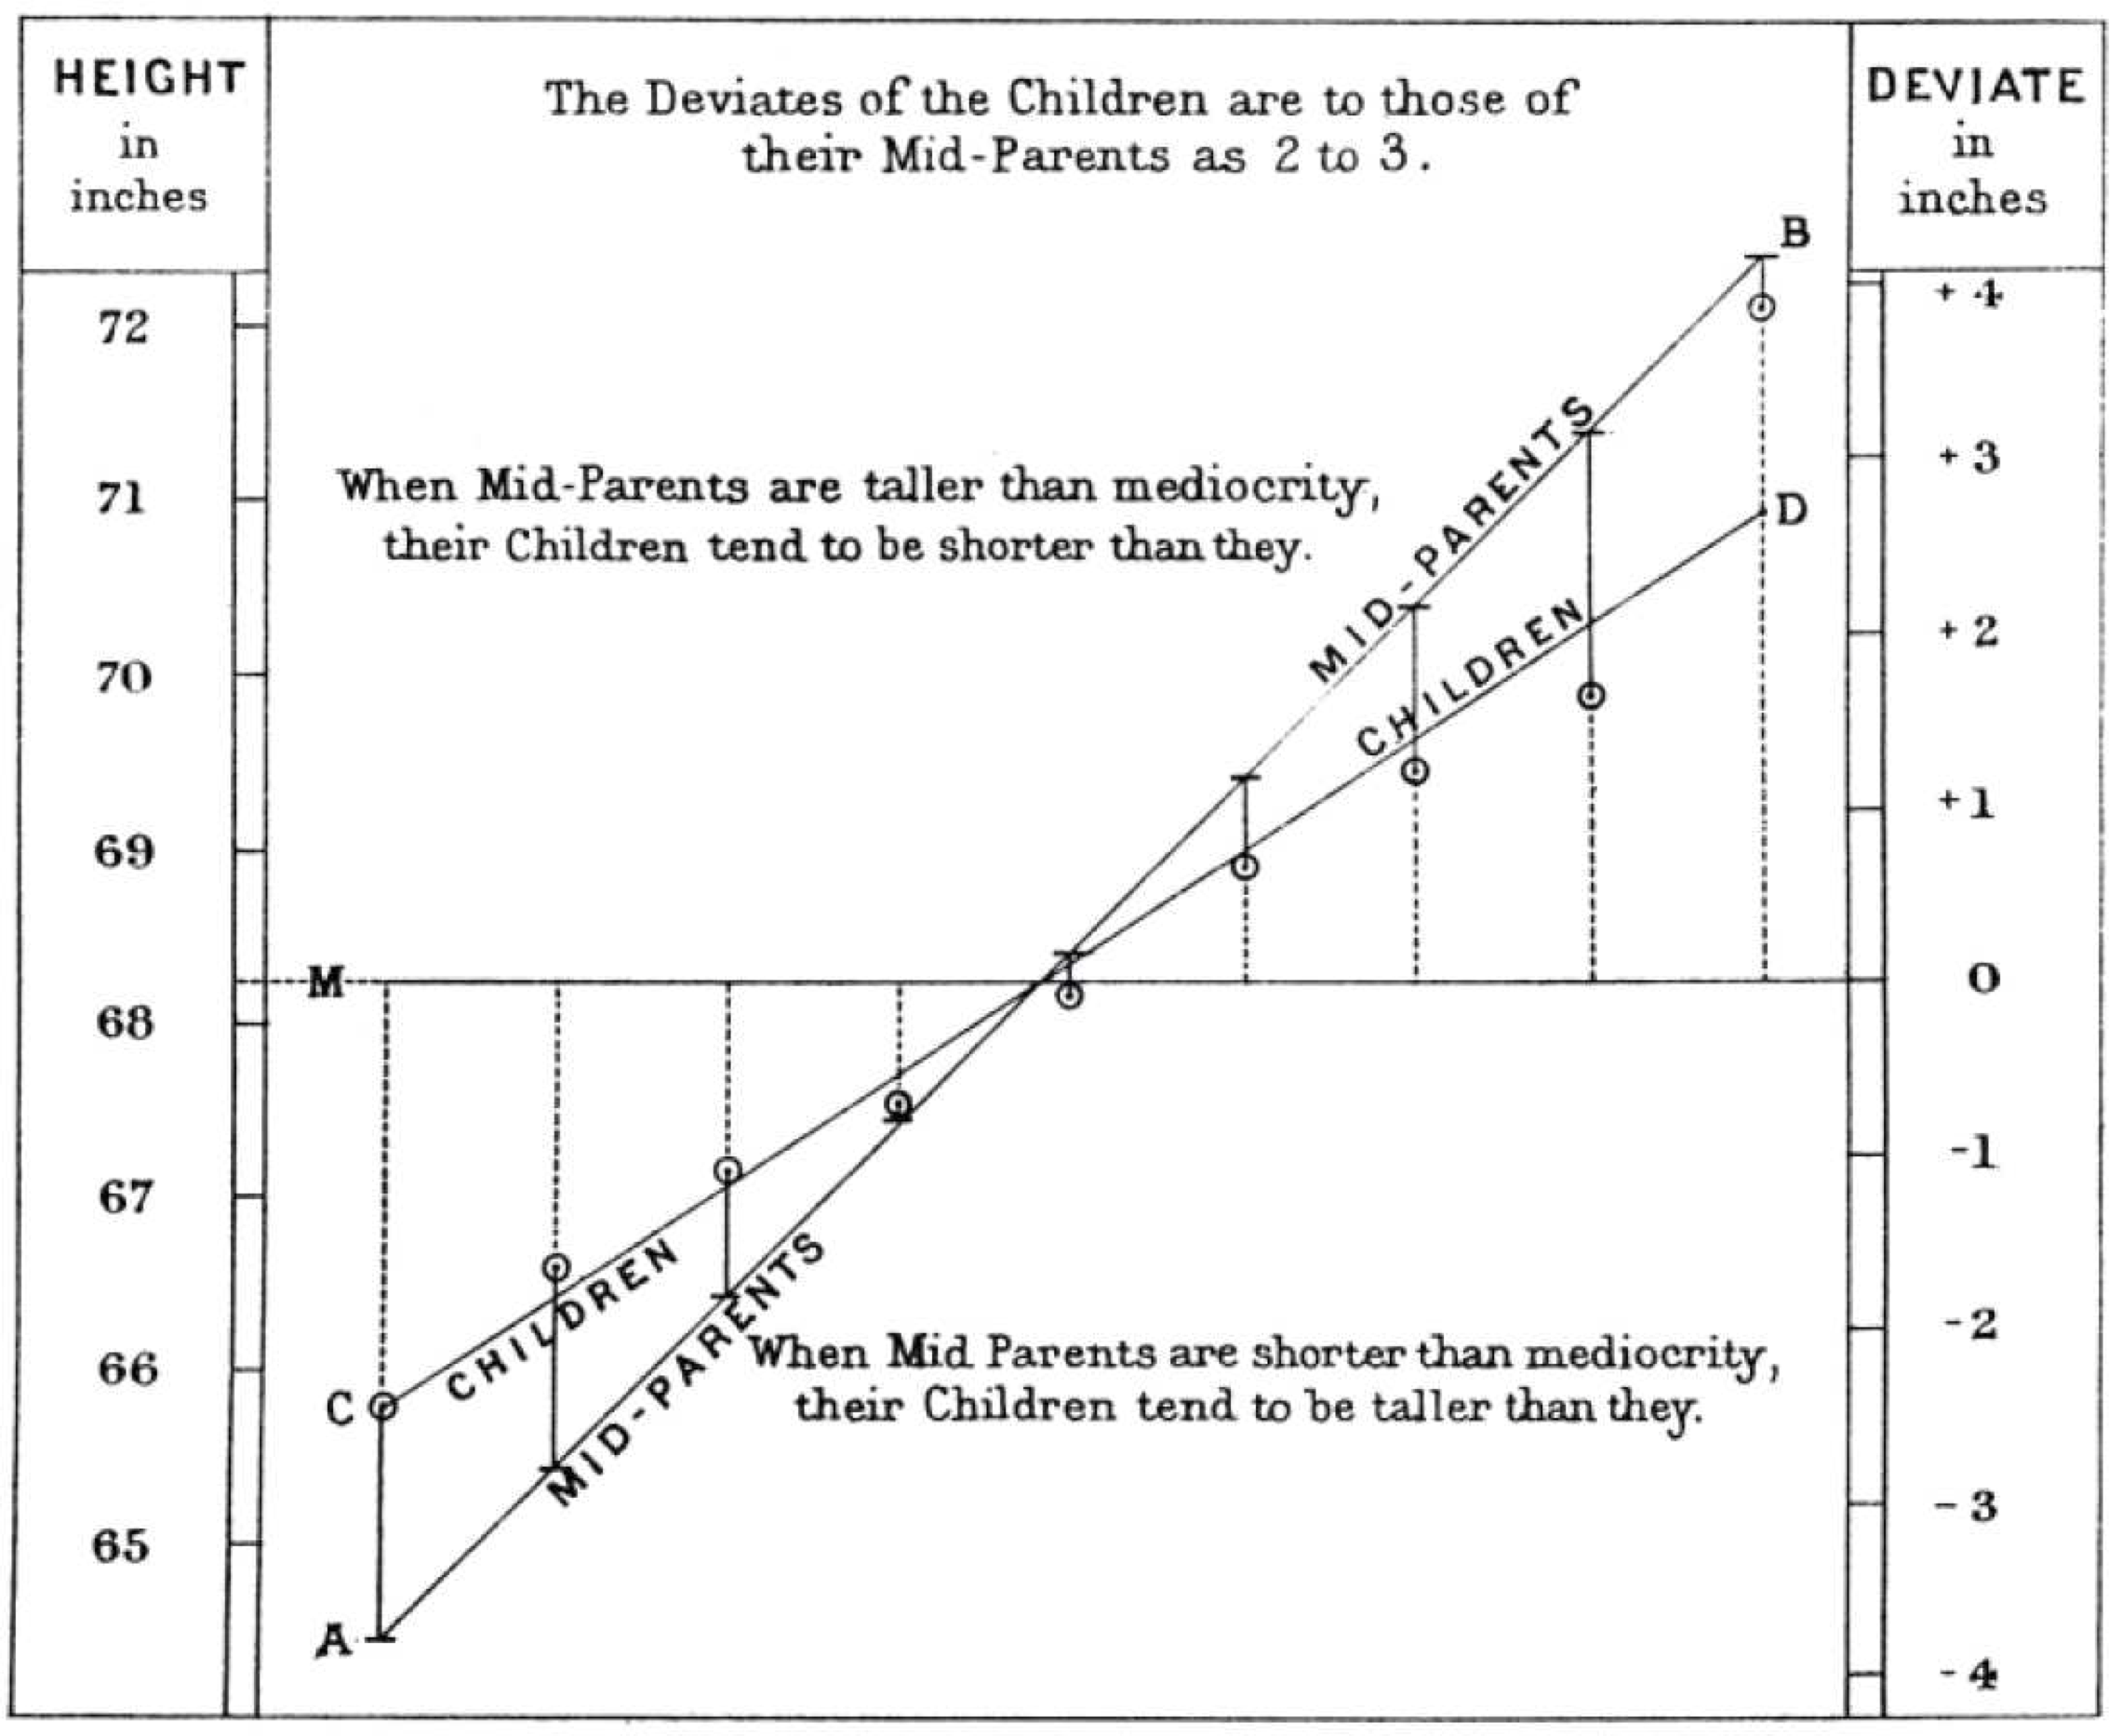
\includegraphics[height=0.6\textheight]{galton.png}
    \end{center}

    $y-\bar{y} \approx \frac{2}{3} \left(x-\bar{x}\right).$
\end{frame}

\begin{frame}{Другие работы Гальтона}
    \begin{center}
            
\includegraphics[width=0.85\textwidth]{galton_other.png}
    \end{center}
\end{frame}

\begin{frame}{Постановка задачи линейной регрессии}
    $1,\dots,n$~--- объекты;

    $x_1,\dots,x_k,y$~--- признаки, значения которых измеряются на объектах;

    $x_1,\dots,x_k$~--- объясняющие переменные (предикторы, регрессоры, факторы, признаки);

    $y$~--- зависимая переменная, отклик.

    \bigskip

    Хотим найти такую функцию $f$, что $y\approx f\left(x_1,\dots,x_k\right)$;

    $$\argmin{f} \mathbb{E}\left(y-f\left(x_1,\dots,x_k\right)\right)^2 = \mathbb{E}\left(y\left|x_1,\dots,x_k\right.\right).$$

    \bigskip

    $\mathbb{E}\left(y\left|x_1,\dots,x_k\right.\right) = f\left(x_1,\dots,x_k\right)$~--- модель регрессии;

    $\mathbb{E}\left(y\left|x_1,\dots,x_k\right.\right) = \beta_0+\sum\limits_{j=1}^k \beta_j x_j$~--- модель линейной регрессии.

    \bigskip

    Здесь и далее $n>k$ ($n\gg k$).
\end{frame}

\begin{frame}{Метод наименьших квадратов (МНК)}
%%%%%%%%%%%%%%%%%%%%%%%%%%%%%%%%%%%%%%%%%%%%%%%%%%%%%%%%%%%%%%%%%%%%%%%
% Для того, чтобы больше не думать про коэффициент b0, можно добавить в матрицу объекты-признаки X единичный столбец. Теперь эта матрица размера n ? (k + 1).
% Задача регрессии будет решаться методом наименьших квадратов без использования регуляризаторов
%%%%%%%%%%%%%%%%%%%%%%%%%%%%%%%%%%%%%%%%%%%%%%%%%%%%%%%%%%%%%%%%%%%%%%%	
	\only<1>{
    Матричные обозначения:
    $$X = \begin{pmatrix}
            x_{10}=1      & x_{11} & \dots  & x_{1k} \\
            \vdots & \vdots & \ddots & \vdots \\
            x_{n0}=1      & x_{n1} & \dots  & x_{nk}
         \end{pmatrix};
    \quad
    y =  \begin{pmatrix}
            y_1 \\ \vdots \\ y_n
         \end{pmatrix};
    \quad
    \beta = \begin{pmatrix}
                \beta_0 \\ \beta_1 \\ \vdots \\ \beta_k
             \end{pmatrix}.
    $$

    \bigskip

    Метод наименьших квадратов:
    \begin{align*}
    & \sum_{i=1}^n \left(y_i - \sum_{j=0}^k \beta_j x_{ij} \right)^2 \rightarrow \min_{\beta}; \\
    & \left\|y-X\beta\right\|_2^2 \rightarrow \min_{\beta}; \\
    & 2X^T\left(y-X\beta\right)=0, \\
    & \hat{\beta} = \left(X^TX\right)^{-1}X^Ty,  \\
    & \hat{y} =  X\left(X^TX\right)^{-1}X^Ty. \\
%    & RSS = \left\|y-X\hat{\beta}\right\|_2^2. \\
    \end{align*}
}
\only<2>{
	МНК в линейной регрессии даёт выборочную оценку линейной аппроксимации условного матожидания $\mathbb{E}\left(y\left|x\right.\right)$
	
	Кроме $\left\|\cdot\right\|_2^2$ это делает любая дивергенция Брегмана:
	$$D\left(y, X\beta\right) = \sum_{i=1}^n \left( \phi\left(y_i\right) - \phi\left(x_i\beta\right) - \phi'\left(x_i\beta\right)\left(y_i-x_i\beta\right)\right),$$
	где $\phi$~--- произвольная непрерывно дифференцируемая выпуклая функция.
	
	\begin{center}
		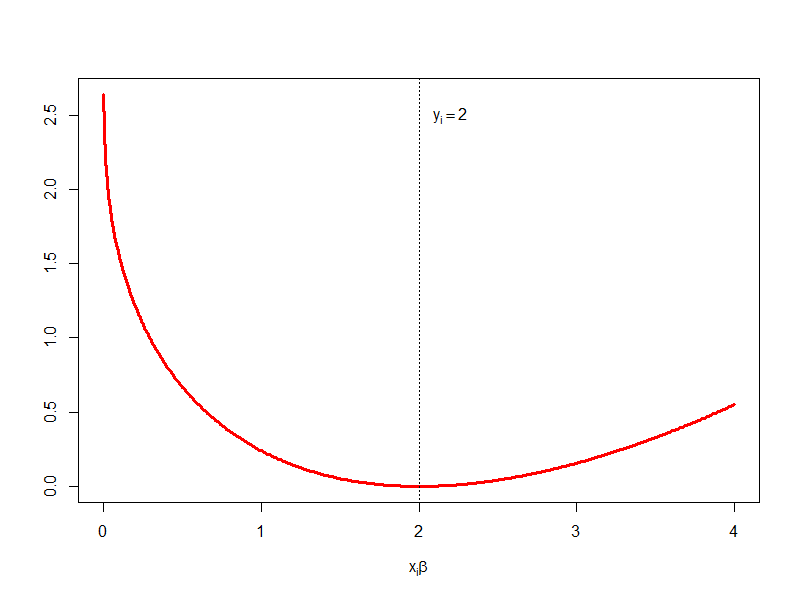
\includegraphics[width=0.35\textwidth]{db1.png}
		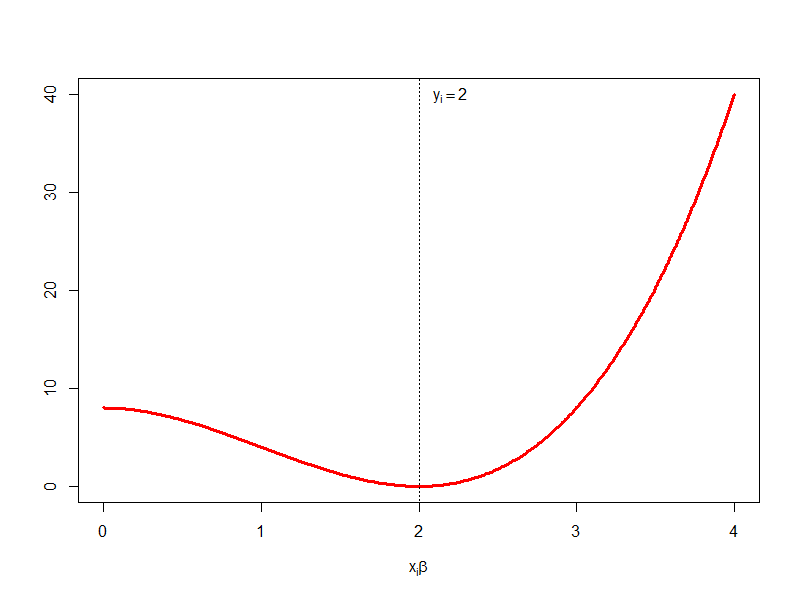
\includegraphics[width=0.35\textwidth]{db2.png}
	\end{center}		
}
\end{frame}

\begin{frame}{Инверсия задачи регрессии}
    \only<1>{
    \begin{block}{Avenhaus et al.}
    Требуется оценить распределение доходов семей, живущих в одном городском квартале по открытым данным. 
    
    Доход семьи --- закрытый показатель, достать который достаточно трудно, согласились огласить доход лишь несколько семей.\\
    Известно, что доход сильно коррелирует со стоимостью недвижимости $\to$ можем построить регрессию и предсказывать независимую переменную по зависимой.
    \end{block}

    
    }
    \only<2>{
    \begin{center}
            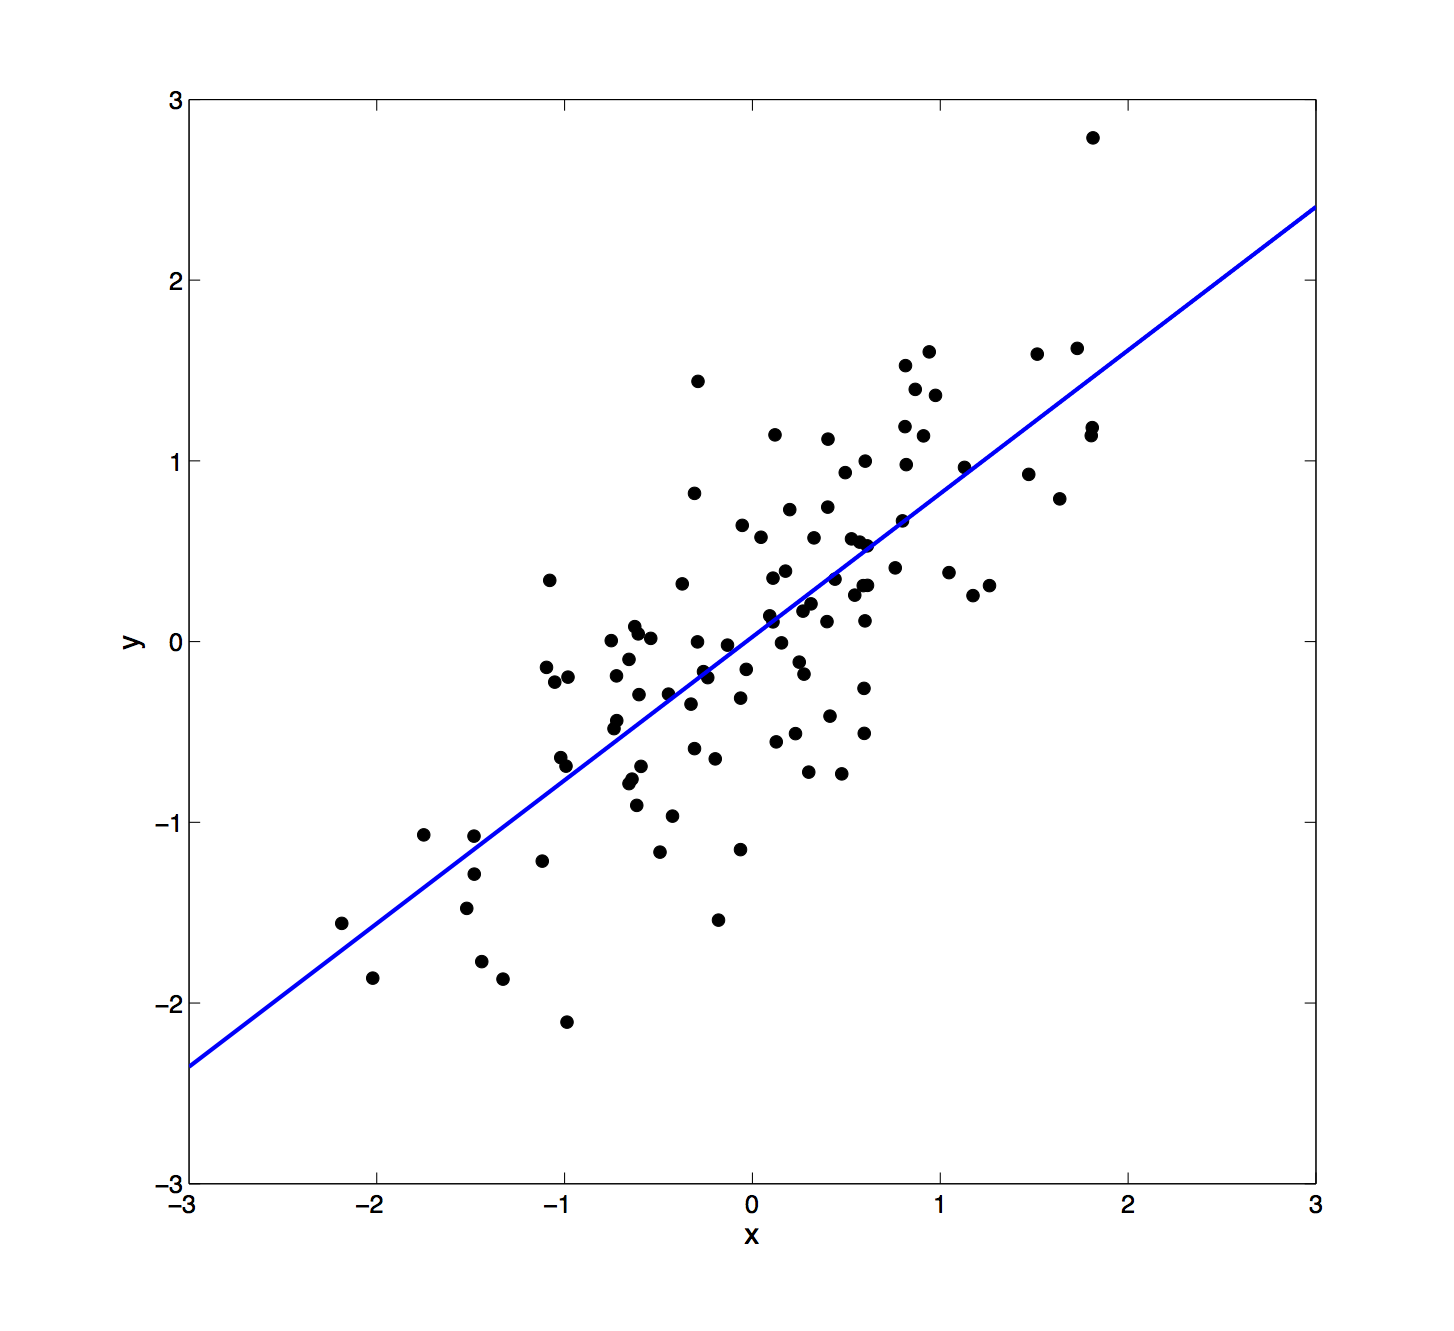
\includegraphics[height=0.8\textheight]{xy2.png}
    \end{center}
    }

    \only<3>{
    \begin{center}
            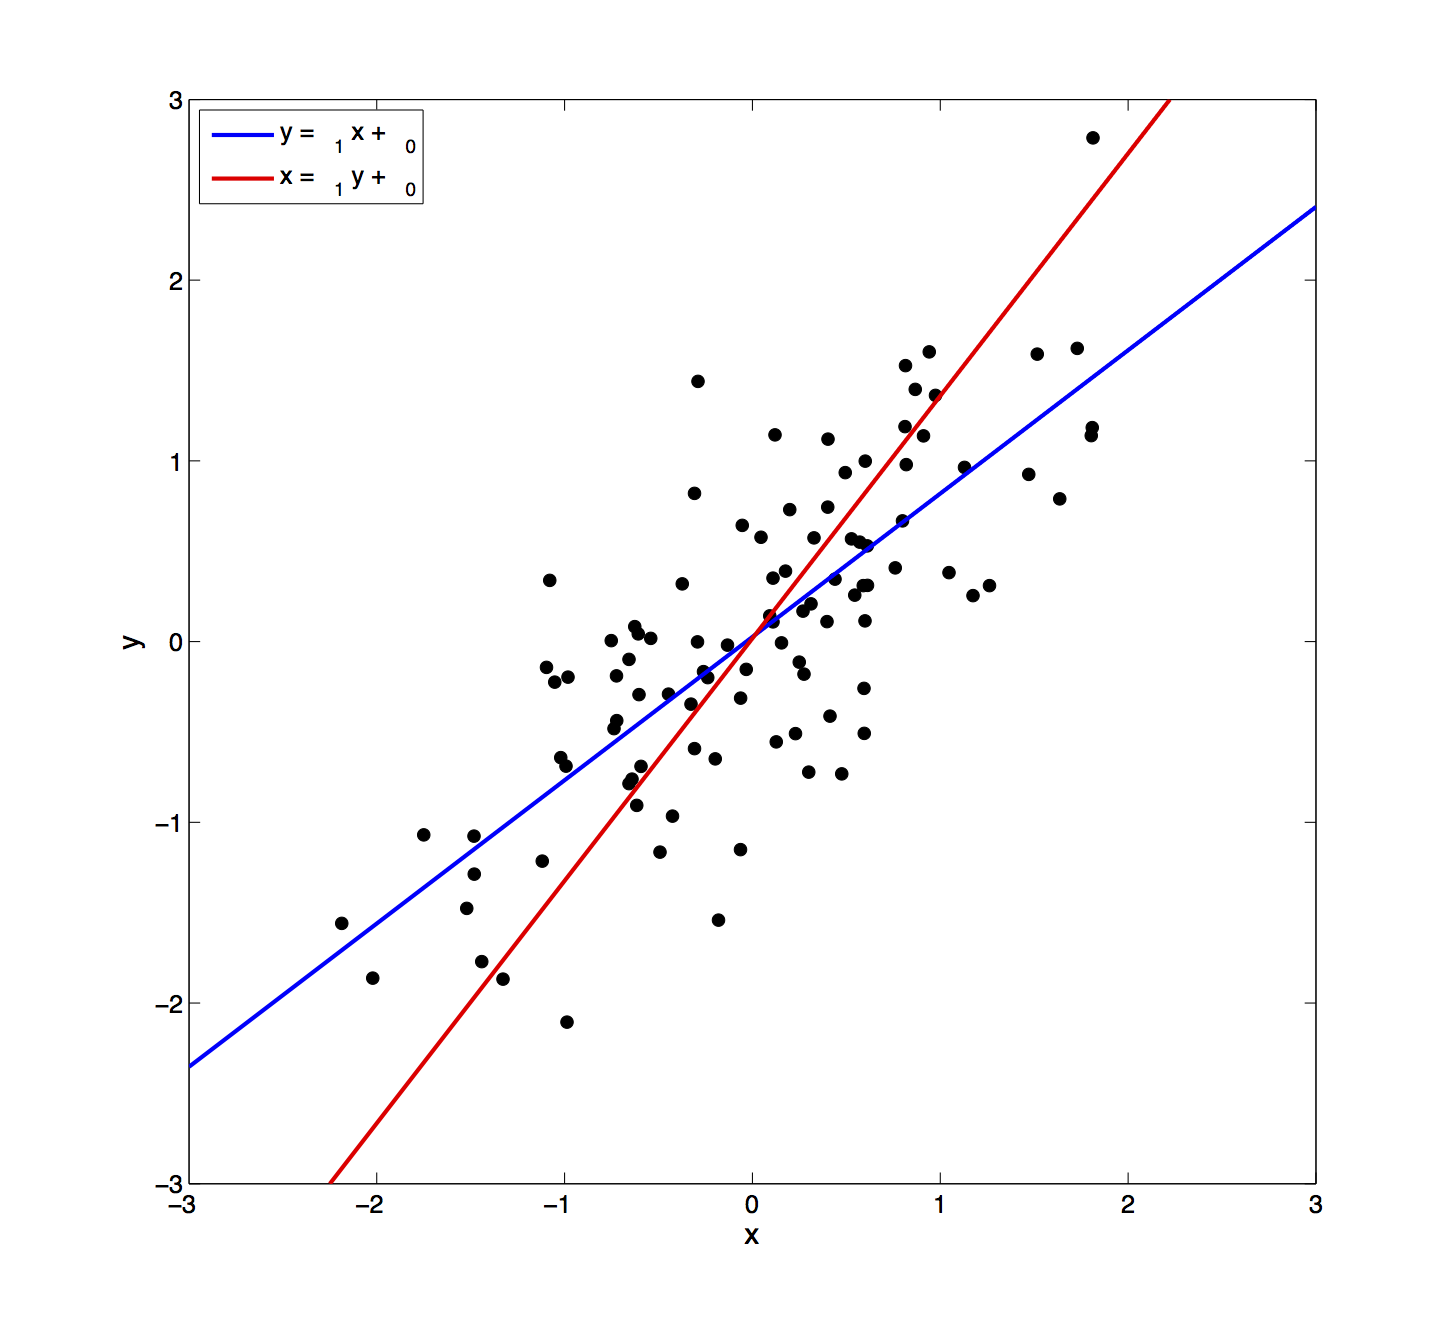
\includegraphics[height=0.8\textheight]{xy3.png}
    \end{center}
    }

    \only<4>{
    \begin{center}
            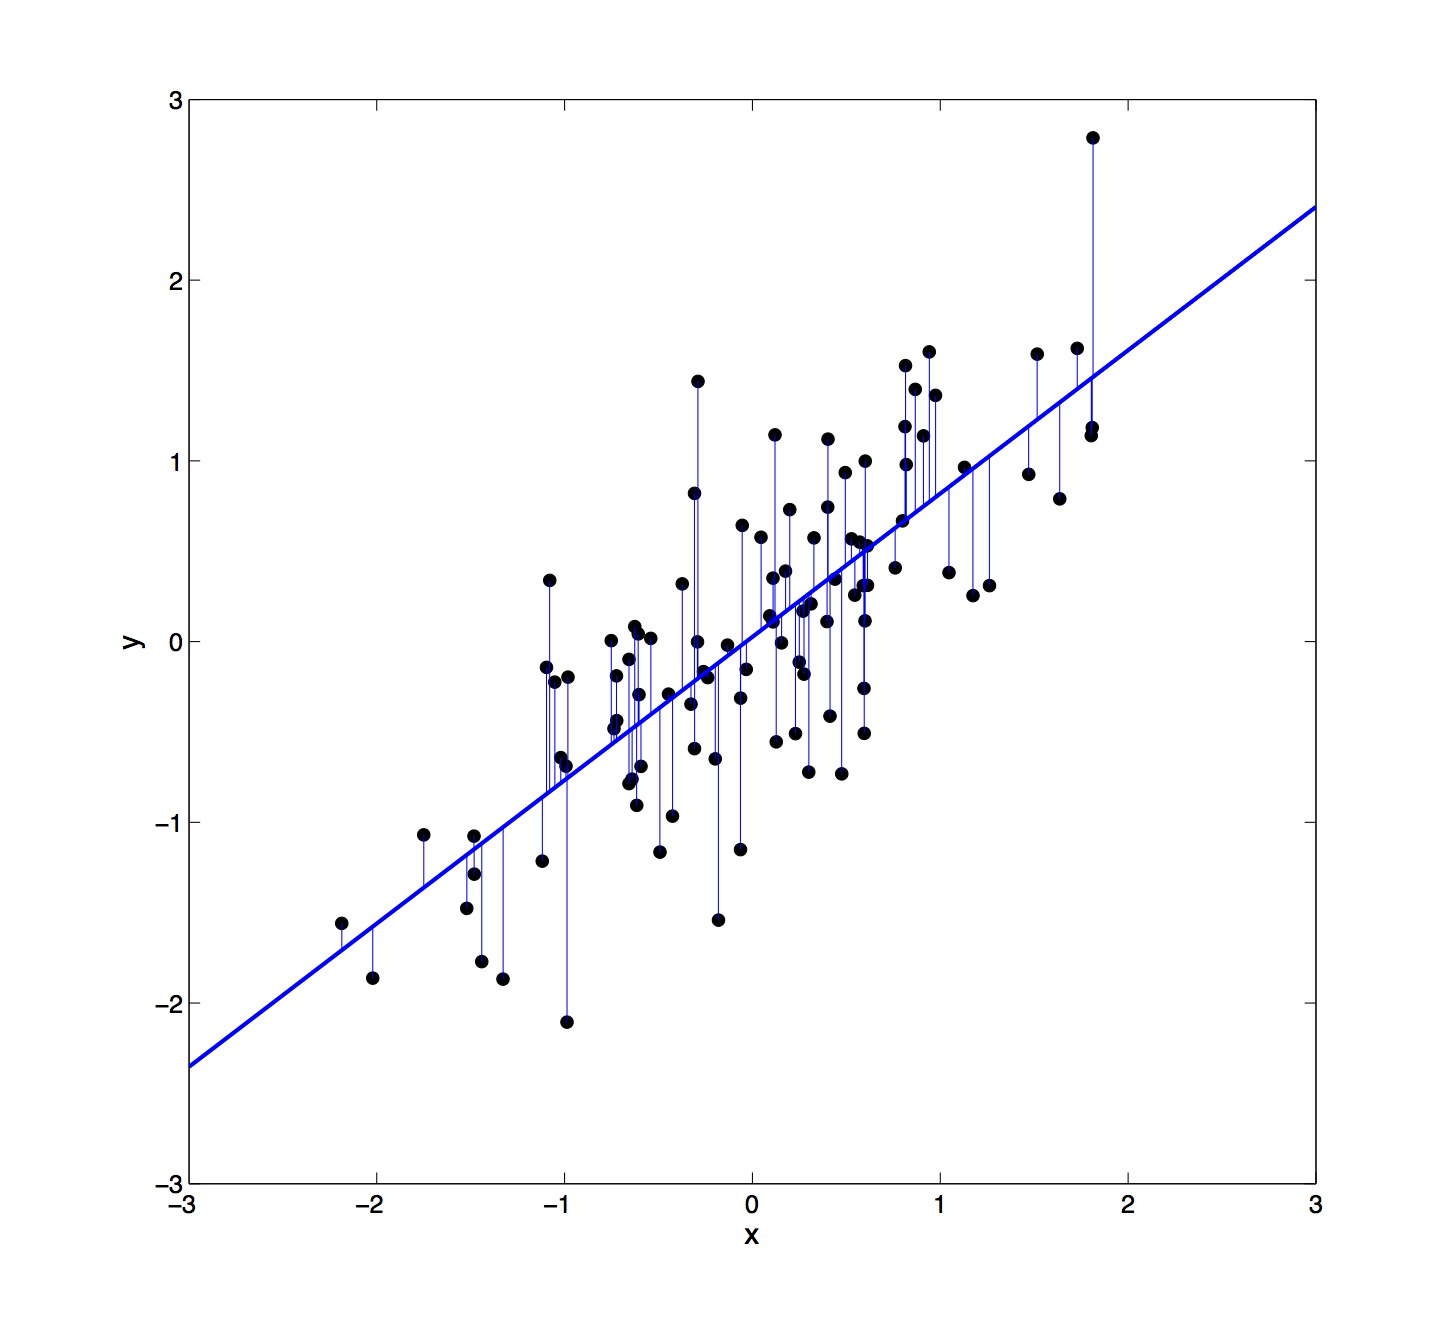
\includegraphics[height=0.8\textheight]{xy4.png}
    \end{center}
    }

    \only<5>{
    \begin{center}
            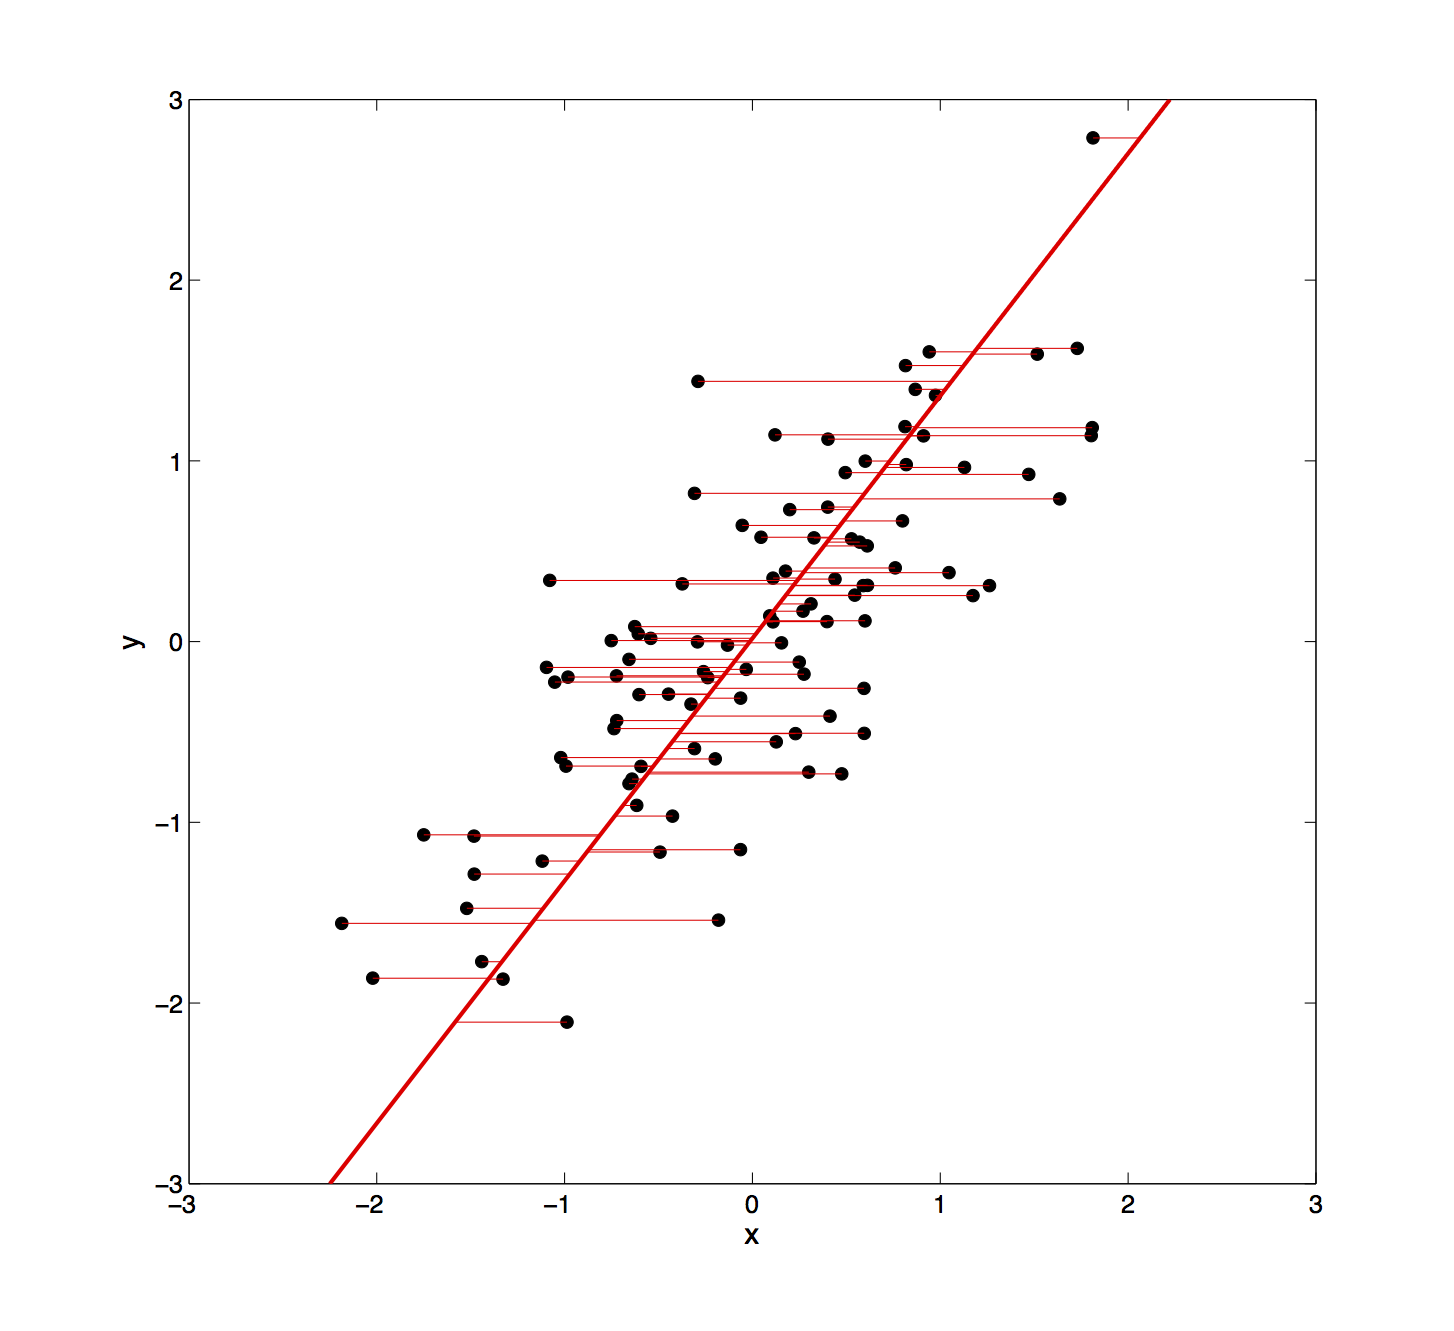
\includegraphics[height=0.8\textheight]{xy5.png}
    \end{center}
    }

    \only<6>{
    \begin{center}
            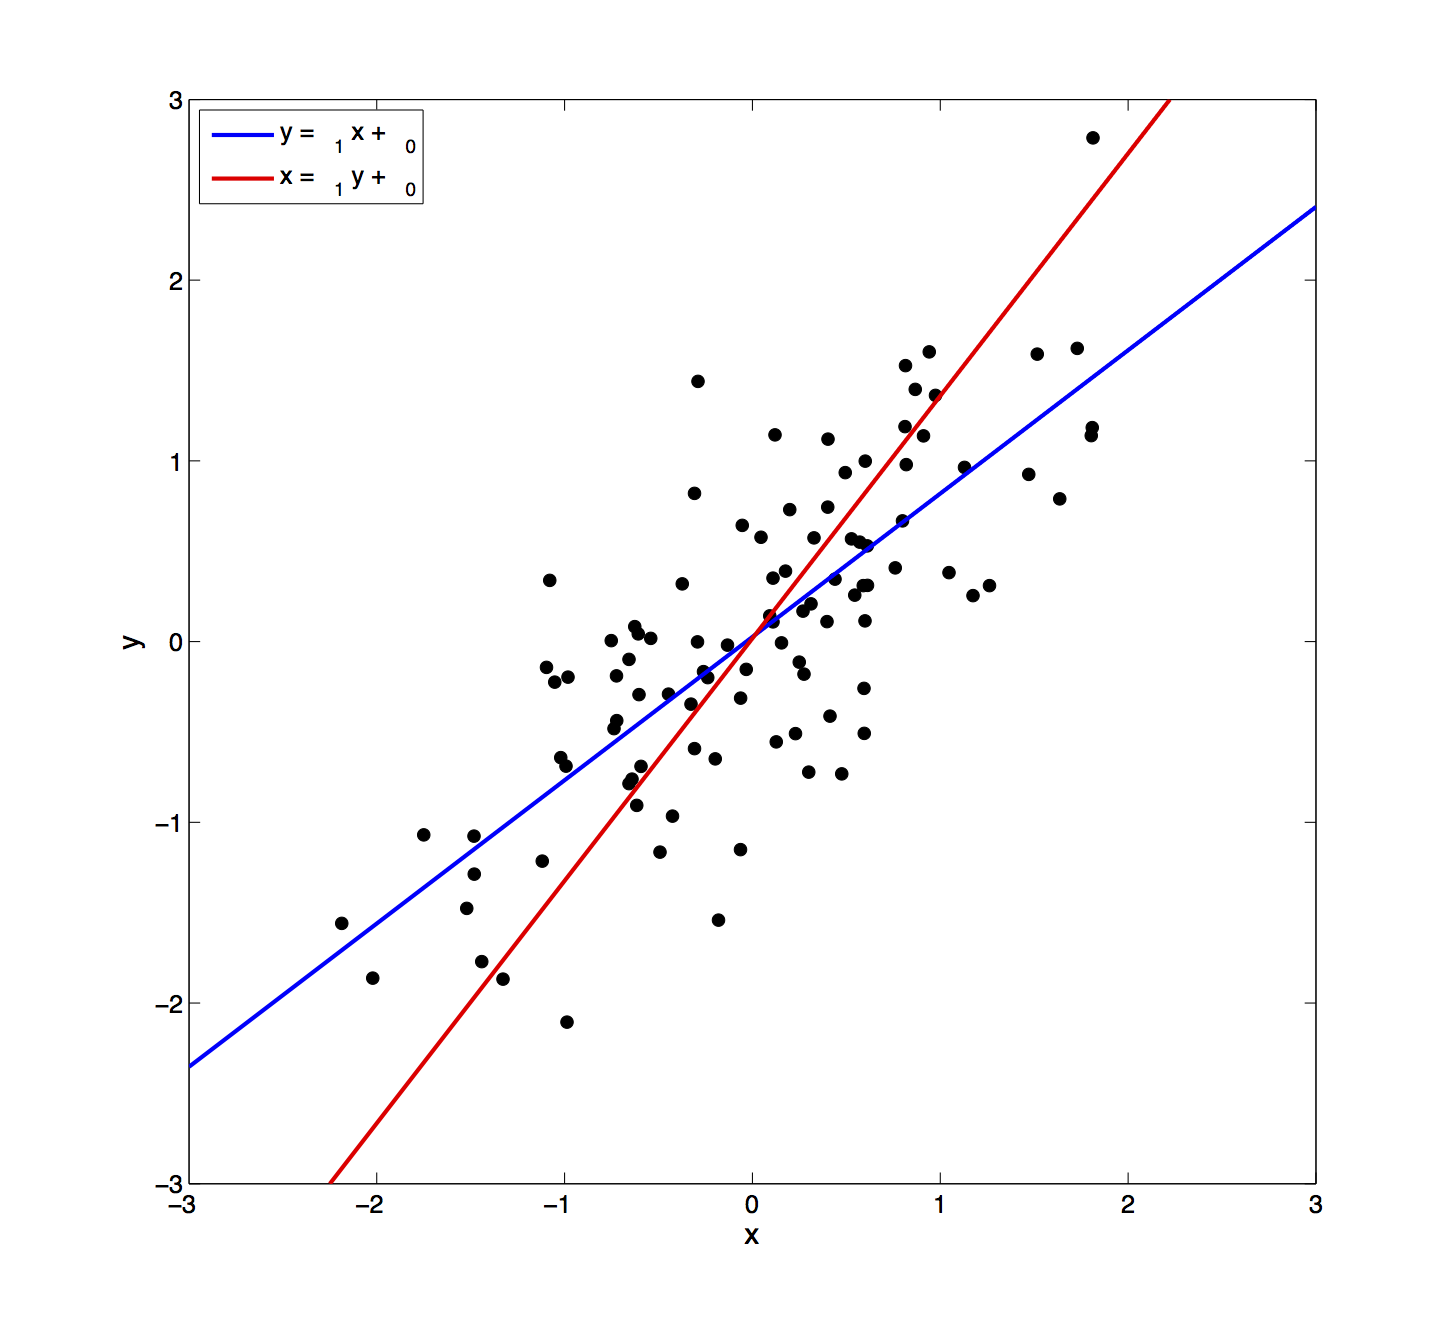
\includegraphics[height=0.3\textheight]{xy3.png}
    \end{center}   
    \begin{itemize}
    \item Две прямые пересекаются в точке $\left(\bar{x},\bar{y}\right).$
    \item Выборочный коэффициент корреляции между $x$ и $y$~--- среднее геометрическое $\hat{\theta}_1$ и $\hat{\phi}_1$: $$\hat{\theta}_1 = \frac{n\sum xy - \sum x \sum y}{n\sum x^2 - \left(\sum x\right)^2}, \;\;\;
    \hat{\phi}_1   = \frac{n\sum xy - \sum x \sum y}{n\sum y^2 - \left(\sum y\right)^2},$$
    $$\hat{r}_{xy}   = \frac{n\sum xy - \sum x \sum y}{\sqrt{\left(n\sum x^2 - \left(\sum x\right)^2\right) \left(n\sum y^2 - \left(\sum y\right)^2 \right)}}.$$    
    \end{itemize}
    }
\end{frame}

\subsection{Свойства МНК-оценок}
\begin{frame}{Goodness-of-fit}
%%%%%%%%%%%%%%%%%%%%%%%%%%%%%%%%%%%%%%%%%%%%%%%%%%%%%%%%%%%%%%%%%%%%%%%
% Чтобы найти качество решения, полученного методом наименьших квадратов, определим величину TSS (Total Sum of Squares) — разброс y относительно своего среднего. этот разброс можно поделить на две части. Одна из частей, ESS - объясненная сумма квадратов, — это сумма квадратов отклонений среднего y от предсказанных y; вторая часть, остаточная сумма квадратов, — это сумма квадратов отклонений предсказанных y от их истинных значений. По этим величинам, ESS и TSS, можно составить меру R2, которая называется коэффициентом детерминации. это доля объясненной дисперсии отклика во всей дисперсии отклика.
%%%%%%%%%%%%%%%%%%%%%%%%%%%%%%%%%%%%%%%%%%%%%%%%%%%%%%%%%%%%%%%%%%%%%%%
    \begin{align*}
    TSS &= \sum_{i=1}^n \left(y_i - \bar{y}\right)^2 \;\; \text{(Total Sum of Squares)}; \\
    ESS &= \sum_{i=1}^n \left(\hat{y}_i - \bar{y}\right)^2 \;\; \text{(Explained Sum of Squares)}; \\
    RSS &= \sum_{i=1}^n \left(y_i - \hat{y}_i\right)^2 \;\; \text{(Residual Sum of Squares)}; \\
    TSS &= ESS + RSS.
    \end{align*}

    \bigskip

    Коэффициент детерминации:
    $$R^2 = \frac{ESS}{TSS} = 1 - \frac{RSS}{TSS}.$$
    $R^2 = r^2_{y\hat{y}}$~--- квадрат коэффициента множественной корреляции $y$~с~$X$.
\end{frame}

\begin{frame}{Приведённый коэффициент детерминации}
    Стандартный коэффициент детерминации всегда увеличивается при добавлении регрессоров в модель, поэтому для отбора признаков его использовать нельзя.

    \bigskip

    Для сравнения моделей, содержащих разное число признаков, можно использовать приведённый коэффициент детерминации:
    $$R^2_a = \frac{ESS/(n-k-1)}{TSS/(n-1)} = 1 - \left(1-R^2\right)\frac{n-1}{n-k-1}.$$
\end{frame}

\begin{frame}{Предположения модели}
%%%%%%%%%%%%%%%%%%%%%%%%%%%%%%%%%%%%%%%%%%%%%%%%%%%%%%%%%%%%%%%%%%%%%%%
% Для того, чтобы решение метода наименьших квадратов обладало интересующими нас свойствами, необходимо сделать следующие предположения.
% 1. истинная модель y действительно линейна: y = X? + ?, где ? — это какая-то ошибка.
% 2. наблюдения, по которым оценивается модель, случайны, то есть объекты представляют собой независимую выборку наблюдений
% 3. матрица X — матрица полного столбцового ранга, то есть ни один из признаков не должен являться линейной комбинацией других. Поскольку среди столбцов есть константа, никакой из признаков в выборке не должен быть константой.
% 4. ошибка случайна
% Уже из этих четырех предположений можно вывести полезное свойство оценок, получаемых методом наименьших квадратов. Если они выполняются, то оценки ?? являются несмещенными и состоятельными оценками истинных ?. 
%%%%%%%%%%%%%%%%%%%%%%%%%%%%%%%%%%%%%%%%%%%%%%%%%%%%%%%%%%%%%%%%%%%%%%%
    \only<1>{
    \begin{enumerate}
    \item Линейность отклика: $y = X\beta+\varepsilon.$
    \item Случайность выборки: наблюдения $(x_i,y_i), i=1,\dots,n$ независимы.
    \item Полнота ранга: ни один из признаков не является константой или линейной комбинацией других признаков ни в популяции, ни в~выборке ($\rank X = k+1$).
    \item Случайность ошибок: $\mathbb{E}\left(\varepsilon\left|X\right.\right) = 0.$
    \end{enumerate}

    \bigskip

    В предположениях (1-4) МНК-оценки коэффициентов $\beta$ являются несмещёнными:
    $$\mathbb{E}\hat{\beta}_j = \beta_j, \; j=0,\dots,k,$$
    и состоятельными:
    $$\forall \gamma>0 \; \lim_{n\rightarrow\infty} P\left(\left|\beta_j-\hat{\beta}_j\right|<\gamma\right) = 1, \; j=0,\dots,k.$$
    }

    \only<2>{
%%%%%%%%%%%%%%%%%%%%%%%%%%%%%%%%%%%%%%%%%%%%%%%%%%%%%%%%%%%%%%%%%%%%%%%
% К четырем предположениям можно добавить еще пятое — предположение гомоскедастичности ошибок: дисперсия ошибки не зависит от значений отклика. Вместе эти пять предположений называются предположениями Гаусса-Маркова. Теорема Гаусса-Маркова утверждает, что если эти предположения выполняются, то МНК-оценки имеют наименьшую дисперсию в классе всех оценок ?, линейных по y. То есть оценки методом наименьших квадратов при выполнении этих пяти предположений в каком-то смысле являются оптимальными.
%%%%%%%%%%%%%%%%%%%%%%%%%%%%%%%%%%%%%%%%%%%%%%%%%%%%%%%%%%%%%%%%%%%%%%%
    \vspace{-18pt}
    \begin{enumerate}
    \item Линейность отклика: $y = X\beta+\varepsilon.$
    \item Случайность выборки: наблюдения $(x_i,y_i), i=1,\dots,n$ независимы.
    \item Полнота ранга: ни один из признаков не является константой или линейной комбинацией других признаков ни в популяции, ни в~выборке ($\rank X = k+1$).
    \item Случайность ошибок: $\mathbb{E}\left(\varepsilon\left|X\right.\right) = 0.$
    \item Гомоскедастичность ошибок: дисперсия ошибки не зависит от~значений признаков: $\mathbb{D}\left(\varepsilon\left|X\right.\right)=\sigma^2.$
    \end{enumerate}
    (предположения Гаусса-Маркова).

    \bigskip

    Теорема Гаусса-Маркова: в предположениях (1-5) МНК-оценки имеют наименьшую дисперсию в классе оценок $\beta$, линейных по $y$.
    }
\end{frame}

\begin{frame}{Неправильное определение модели}
	\textbf{Недоопределение}: если зависимая переменная определяется моделью
	$$y = \beta_0+\beta_1x_1 + \dots+\beta_{j-1}x_{j-1} + \beta_j x_j + \beta_{j+1} x_{j+1} + \dots + \beta_k x_k + \varepsilon,$$
	а вместо этого используется модель
	$$y = \beta_0+\beta_1x_1 + \dots+\beta_{j-1}x_{j-1} + \beta_{j+1} x_{j+1} + \dots + \beta_k x_k+\varepsilon,$$
	то МНК-оценки $\hat{\beta}_0,\dots,\hat{\beta}_{j-1},\hat{\beta}_{j+1},\dots,\hat{\beta}_k$ являются смещёнными и~несостоятельными оценками $\beta_0,\dots,\beta_{j-1},\beta_{j+1},\dots,\beta_k.$
	
	\bigskip
	
	\textbf{Переопределение}: если признак $x_j$ не влияет на $y$, т.\,е. $\beta_j=0$, то~МНК-оценка $\hat{\beta}$ остаётся несмещённой состоятельной оценкой $\beta$, но~дисперсия её возрастает.
\end{frame}

\begin{frame}{Дисперсия $\hat{\beta}_j$}
    \only<1>{
%%%%%%%%%%%%%%%%%%%%%%%%%%%%%%%%%%%%%%%%%%%%%%%%%%%%%%%%%%%%%%%%%%%%%%%
% Из сделанных предположений вытекает следующее выражение для дисперсии МНК-оценок. то есть:
% • чем больше ?2, тем больше дисперсия ??j;
% • чем больше вариация значений xj в выборке, тем меньше дисперсия ??j;
% • чем лучше признак xj объясняется линейной комбинацией оставшихся признаков, тем больше дисперсия ?? j .
%%%%%%%%%%%%%%%%%%%%%%%%%%%%%%%%%%%%%%%%%%%%%%%%%%%%%%%%%%%%%%%%%%%%%%%
    В предположениях (1-5) дисперсии МНК-оценок коэффициентов $\beta$ задаются следующим образом:
    $$\mathbb{D}\left(\left.\hat{\beta}_j\right|X\right) = \frac{\sigma^2}{TSS_j \left(1-R^2_j\right)},$$
    где $TSS_j = \sum\limits_{i=1}^n \left(x_{ij}-\bar{x}_j\right)^2,$\; $R_j^2$~--- коэффициент детерминации при регрессии $x_j$ на все остальные признаки из $X$.
    
    \bigskip
    
    \begin{itemize}
    \item Чем больше дисперсия ошибки $\sigma^2$, тем больше дисперсия оценки $\hat{\beta}_j$.
    \item Чем больше вариация значений признака $x_j$ в выборке, тем меньше дисперсия оценки $\hat{\beta}_j$.
    \item Чем лучше признак $x_j$ объясняется линейной комбинацией оставшихся признаков, тем больше дисперсия оценки $\hat{\beta}_j$.
    \end{itemize}

    }

    \only<2>{    
%%%%%%%%%%%%%%%%%%%%%%%%%%%%%%%%%%%%%%%%%%%%%%%%%%%%%%%%%%%%%%%%%%%%%%%
% По предположению о полноте столбцового ранга матрицы X коэффициент детерминации Rj2 < 1, но, тем не менее, может быть Rj2 ? 1. Такая ситуация называется мультиколлинеарностью.
% В матричном виде выражение для дисперсии вектора ?? выглядит вот так: 
% Если матрица X содержит столбцы, которые почти линейно зависимы, то матрица XT X будет плохо обуслов- лена. При обращении этой матрицы будет получаться численная неустойчивость, поэтому дисперсия оценок ??j будет велика.
% Следует обратить внимание, что определение мультиколлинеарности не включает случай, когда столбцы полностью линейно зависимы. Мультиколлинеарность — это близкая к линейной зависимость признаков.
%%%%%%%%%%%%%%%%%%%%%%%%%%%%%%%%%%%%%%%%%%%%%%%%%%%%%%%%%%%%%%%%%%%%%%%
    $R_j^2<1$ по предположению (3); тем не менее, может быть $R^2_j\approx1.$
    	
    \bigskip
    	
    В матричном виде:
    $$\mathbb{D}\left(\left.\hat{\beta}\right|X\right) = \sigma^2\left(X^TX\right)^{-1}.$$
    Если столбцы $X$ почти линейно зависимы, то матрица $X^TX$ плохо обусловлена, и дисперсия оценок $\hat{\beta}_j$ велика.

    \bigskip

    Близкая к линейной зависимость между двумя или более признаками $x_j$ называется \textbf{мультиколлинеарностью}.
    
    Проблема мультиколлинеарности решается с помощью отбора признаков или использования регуляризаторов.
    }
\end{frame}

\subsection{Категориальные признаки}
\begin{frame}{Бинарные признаки}
	Если $x_j$ принимает только два значения, то они кодируются нулём и~единицей. Например, если $x_j$~--- пол испытуемого, то можно задать $x_j = \left[\text{пол = мужской}\right].$
	
	\bigskip
	
	Механизм построения регрессии не меняется.
\end{frame}

\begin{frame}{Категориальные признаки}
	Как кодировать дискретные признаки $x_j$, принимающие более двух значений?
	
	Пусть $y$ --- средний уровень заработной платы, $x$ --- тип должности (рабочий / инженер / управляющий).
	Допустим, мы закодировали эти должности следующим образом:
	\begin{center}
		\begin{tabular}{|l|c|} \hline
			Тип должности & $x$ \\\hline
			рабочий       & $1$ \\
			инженер       & $2$ \\
			управляющий   & $3$ \\\hline
		\end{tabular}
	\end{center}
	и построили регрессию $y=\beta_0+\beta_1x$. Тогда для рабочего, инженера и~управляющего ожидаемые средние уровни заработной платы определяются следующим образом:
	\begin{align*}
	y_{bc} &= \beta_0 + \beta_1, \\
	y_{pr} &= \beta_0 + 2\beta_1, \\
	y_{wc} &= \beta_0 + 3\beta_1.
	\end{align*}
	Согласно построенной модели, разница в средних уровнях заработной платы рабочего и~инженера в точности равна разнице между зарплатами инженера и~управляющего.
\end{frame}

\begin{frame}{Фиктивные переменные}
	Верный способ использования категориальных признаков в регрессии~--- введение бинарных фиктивных переменных (dummy variables).
	
	Пусть признак $x_j$ принимает $m$ различных значений, тогда для его кодирования необходима $m-1$ фиктивная переменная.
	
	\bigskip
	
	Способы кодирования:
	\begin{center}
		\begin{tabular}{|l|cc|cc|} \hline
			& \multicolumn{2}{c|}{Dummy}  & \multicolumn{2}{c|}{Deviation} \\\hline
			Тип должности &$x_1$&$x_2$&$x_1$&$x_2$ \\\hline
			рабочий       & $0$ & $0$ & $1$ & $0$ \\
			инженер       & $1$ & $0$ & $0$ & $1$ \\
			управляющий   & $0$ & $1$ &$-1$ &$-1$ \\ \hline
		\end{tabular}
	\end{center}
	
	\bigskip
	
	$$y = \beta_0 + \beta_1x_1 + \beta_2x_2$$
	
	\begin{itemize}
		\item При dummy-кодировании коэффициенты $\beta_1,\beta_2$ оценивают среднюю разницу в уровнях зарплат инженера и управляющего с рабочим.
		\item При deviation-кодировании коэффициенты $\beta_1,\beta_2$ оценивают среднюю разницу в уровнях зарплат рабочего и инженера со средним по всем должностям.
	\end{itemize}
\end{frame}

\section{Анализ моделей}
\begin{frame}{Вопросы}
    \begin{enumerate}
    \item Как найти доверительные интервалы для $\beta_j$ и проверить гипотезу $H_0\colon \beta_j=0$?
    \item Как найти доверительный интервал для значений отклика на новом объекте $y(x_0)$?
    \item Как проверить адекватность построенной модели?
    \end{enumerate}
\end{frame}

\subsection{Предположение о нормальности ошибок}
\begin{frame}{Предположение о нормальности ошибок}
%%%%%%%%%%%%%%%%%%%%%%%%%%%%%%%%%%%%%%%%%%%%%%%%%%%%%%%%%%%%%%%%%%%%%%%
% К 5 предположениям Гаусса-Маркова можно добавить еще одно, предположение о нормальности ошибки. Если выполняются эти 6 предположений, то оценки, даваемые методом наименьших квадратов, совпадают с оценками максимального правдоподобия. Это открывает доступ к прекрасным свойствам оценок макси- мального правдоподобия. Из этих 6 предположений вытекает, что оценки метода наименьших квадратов, во-первых, имеют наименьшую дисперсию среди всех несмещенных оценок ?. Во-вторых, имеют нормальное распределение. Далее, дисперсию шума можно оценить с помощью RSS. Кроме того, отношение RSS к истинной дисперсии будет распределено по хи квадрат. Наконец, следующее очень сильное свойство. Для любого вещественного вектора c длины k + 1 справедливо следующее утверждение
%%%%%%%%%%%%%%%%%%%%%%%%%%%%%%%%%%%%%%%%%%%%%%%%%%%%%%%%%%%%%%%%%%%%%%%
    \only<1>{
    \begin{enumerate}\setcounter{enumi}{5}
    \item Нормальность ошибок: $\varepsilon\left| X\right. \sim N\left(0,\sigma^2\right).$
    \end{enumerate}
	Эквивалентная запись: $y\left|X\right.\sim N\left(X\beta,\sigma^2\right).$
	
    \bigskip

    \begin{itemize}
    \item В предположениях (1-6) МНК-оценки совпадают с оценками максимального правдоподобия.
    \end{itemize}

    ММП:
    \begin{align*}
    & p\left(\varepsilon_i\right) = \frac1{ \sqrt{2\pi} \sigma} e^{-\frac1{2\sigma}\varepsilon^2_i}, \\
    & \ln \prod_{i=1}^n p\left(\varepsilon_i\right) \rightarrow \max_{\beta}, \\
    & \sum_{i=1}^n \left(-\frac1{2}\ln\left(2\pi\sigma\right) - \frac1{2\sigma}\varepsilon_i^2\right) \rightarrow \max_{\beta}, \\
    & \sum_{i=1}^n \varepsilon_i^2 = \sum_{i=1}^n \left(y_i - \sum_{j=0}^k \beta_j x_{ij} \right)^2 \rightarrow \min_{\beta}.
    \end{align*}
    }

    \only<2>{
    \begin{itemize}
    \item МНК-оценки $\hat{\beta}$ имеют наименьшую дисперсию среди всех несмещённых оценок $\beta$.
    \item МНК-оценки $\hat{\beta}$ имеют нормальное распределение $N\left(\beta, \sigma^2\left(X^TX\right)^{-1}\right).$
    \item Несмещённой оценкой $\sigma^2$ является $$\hat{\sigma}^2 = \frac1{n-k-1} RSS;$$
          кроме того, $\frac1{\sigma^2}RSS\sim\chi^2_{n-k-1}.$
    \item $\forall c \in \mathbb{R}^{k+1}$ $$\frac{c^T \left(\beta-\hat{\beta}\right)}{\hat{\sigma} \sqrt{c^T \left(X^TX\right)^{-1}c}}\sim St(n-k-1).$$
    \end{itemize}
    }
\end{frame}

\subsection{Доверительные интервалы и проверка гипотез}
\begin{frame}{Доверительные и предсказательные интервалы}
%%%%%%%%%%%%%%%%%%%%%%%%%%%%%%%%%%%%%%%%%%%%%%%%%%%%%%%%%%%%%%%%%%%%%%%
% Если выполняются описанные предположения, то можно строить доверительный интервалы для коэффициентов ?j , доверительные интервалы для среднего отклика E (y |x ) и предсказательные интервалы для значения y |x. 
% Во-первых, 100(1 ? ?)% доверительный интервал для дисперсии шума ?2 можно построить через отношение RSS к квантилям распределения ?2:
% Во-вторых, чтобы построить доверительные интервалы для коэффициента ?j, можно использовать послед- нее утверждение (о распределении Стьюдента), и в качестве вектора c выбрать вектор, состоящий из всех нулей, в котором на j позиции стоит 1. Тогда 100(1 ? ?)% доверительный интервал для j коэффициента ?j задаётся следующим образом:
% Чтобы построить доверительный интервал для математического ожидания отклика y на новом объекте, за- даваемом вектором x0, в качестве вектора c можно использовать x0. 100(1 ? ?)% доверительный интервал для E (y |x0 ) готов:
% Чтобы построить предсказательный интервал для значения отклика на этом же самом объекте y(x0) = xT0 ? + ? (x0 ), необходим дополнительно учесть ещё дисперсию ошибки. Формула для предсказательного интервала отличается от формулы для доверительного интервала условного математического ожидания только единицей, стоящей под корнем.
%%%%%%%%%%%%%%%%%%%%%%%%%%%%%%%%%%%%%%%%%%%%%%%%%%%%%%%%%%%%%%%%%%%%%%%
    $100(1-\alpha)$\% доверительный интервал для $\sigma$:
    $$\sqrt{\frac{RSS}{\chi^2_{n-k-1,1-\alpha/2}}} \leq \sigma \leq \sqrt{\frac{RSS}{\chi^2_{n-k-1,\alpha/2}}}.$$

    \bigskip

    Возьмём $c=\left(0\dots0\underset{j}{1}0\dots0\right);$ \; $100(1-\alpha)\%$ доверительный интервал для~$\beta_j$:
    $$\hat{\beta}_j \pm t_{n-k-1,1-\alpha/2}\hat{\sigma} \sqrt{\left(X^TX\right)^{-1}_{jj}}.$$

	\bigskip

    Для нового объекта $x_0$ возьмём $c=x_0;$ \; $100(1-\alpha)\%$ доверительный интервал для $\mathbb{E}\left(y\left|\right.x=x_0\right)=x_0^T\beta$:
    $$x_0^T \hat{\beta} \pm t_{n-k-1,1-\alpha/2}\hat{\sigma} \sqrt{x_0^T \left(X^TX\right)^{-1} x_0}.$$

    \bigskip
    
    Чтобы построить предсказательный интервал для $y\left(x_0\right) = x_0^T\beta + \varepsilon\left(x_0\right),$ учтём ещё дисперсию ошибки:
    $$x_0^T \hat{\beta} \pm t_{n-k-1,1-\alpha/2}\hat{\sigma} \sqrt{1 + x_0^T \left(X^TX\right)^{-1} x_0}.$$
\end{frame}

\begin{frame}{t-критерий Стьюдента}
    \only<1>{
    \begin{center}
        \begin{tabular}{rl}
            нулевая гипотеза:               & $H_0\colon \beta_j=0$ \\
            альтернатива:                   & $H_1\colon \beta_j<\neq>0$ \\
            статистика:                     & $T = \frac{\hat{\beta}_j}{ \sqrt{ \frac{RSS}{n-k-1} \left(X^TX\right)^{-1}_{jj}}}$ \\
            нулевое распределение:          & $St(n-k-1)$\\
        \end{tabular}
        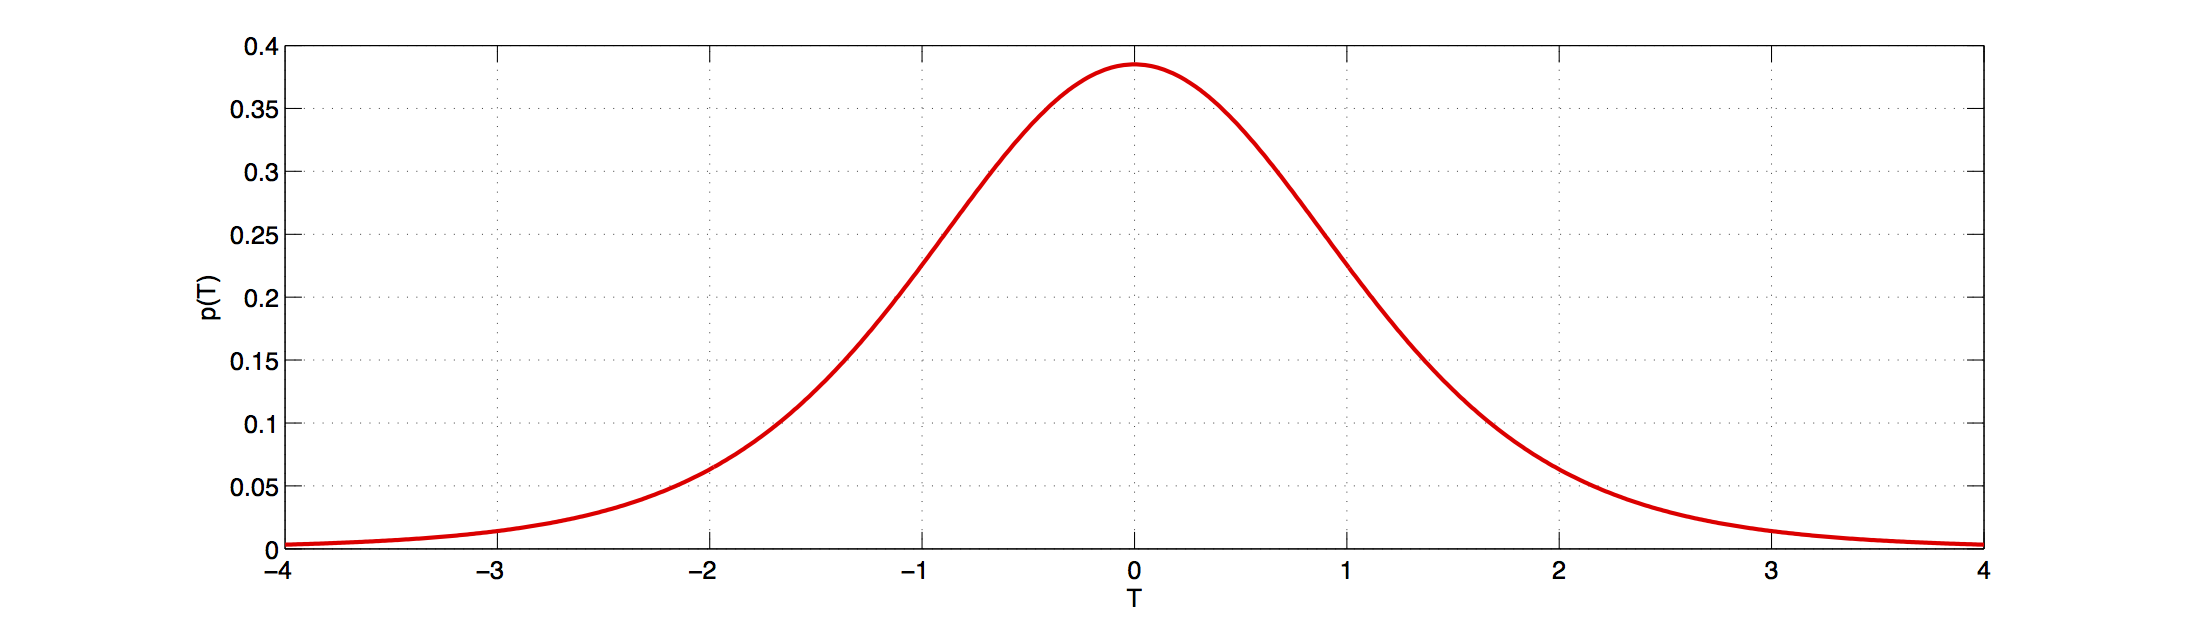
\includegraphics[width=0.85\textwidth]{stud.png}    
    \end{center}
     }

     \only<2>{
     \textbf{Пример:} имеется 12 испытуемых, $x$~---  результат прохождения испытуемым составного теста скорости реакции, $y$~--- результат его теста на симулятора транспортного средства. Проведение составного теста значительно проще и требует меньших затрат, поэтому ставится задача предсказания $y$ по $x$, для чего строится линейная регрессия согласно модели
        $$y = \beta_0 + \beta_1x + \varepsilon.$$
    Значима ли переменная $x$ для предсказания $y$?

    \bigskip

    $H_0\colon \beta_1 = 0.$

    $H_1\colon \beta_1 \neq 0$  $\Rightarrow p = 2.2021 \times 10^{-5}$.
     }
\end{frame}

\begin{frame}{t-критерий Стьюдента}
    \only<1>{
    \begin{center}
        \begin{tabular}{rl}
            нулевая гипотеза:               & $H_0\colon \beta_j=a$ \\
            альтернатива:                   & $H_1\colon \beta_j<\neq>a$ \\
            статистика:                     & $T = \frac{\hat{\beta}_j-a}{\sqrt{\frac{RSS}{n-k-1}\left(X^TX\right)^{-1}_{jj}}}$ \\
            нулевое распределение:          & $St(n-k-1)$\\
        \end{tabular}
        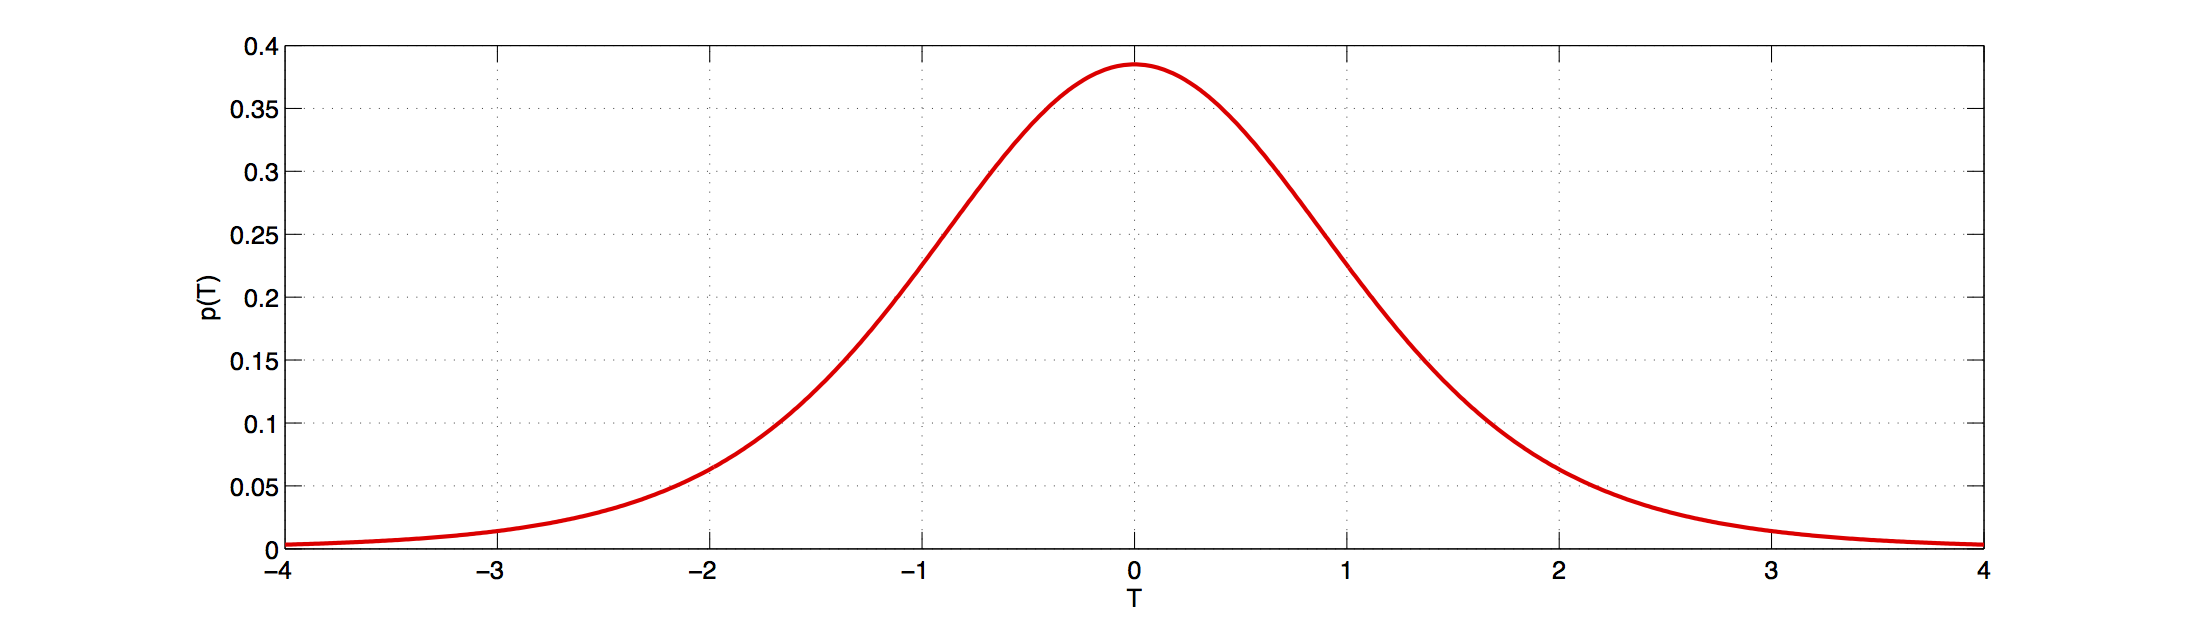
\includegraphics[width=0.85\textwidth]{stud.png}    
    \end{center}
     }

     \only<2>{
     \textbf{Пример:} по выборке из 506 жилых районов, расположенных в пригородах Бостона, строится модель средней цены на жильё следующего вида:
        $$\ln price = \beta_0 + \beta_1 \ln nox + \beta_2 \ln dist + \beta_3 rooms + \beta_4 stratio + \varepsilon,$$
     где $nox$~---  содержание в воздухе двуокиси азота, $dis$~--- взвешенное среднее расстояние от жилого района до пяти основных мест      трудоустройства, $rooms$~---  среднее число комнат в доме жилого района, $stratio$~---  среднее отношения числа студентов к числу учителей в школах района.

      Коэффициент $\beta_1$ имеет смысл эластичности цены по признаку $nox$. По~экономическим соображениям интерес представляет гипотеза о том, что эластичность равна $-1$.

    \bigskip

    $H_0\colon \beta_1 = -1.$

    $H_1\colon \beta_1 \neq -1$  $\Rightarrow p = 0.6945$.
     }
\end{frame}

\begin{frame}{Критерий Фишера}
%%%%%%%%%%%%%%%%%%%%%%%%%%%%%%%%%%%%%%%%%%%%%%%%%%%%%%%%%%%%%%%%%%%%%%%
% Для проверки гипотезы о том, что сразу несколько коэффициентов модели равны 0, будет использоваться не критерий Стьюдента, а критерий Фишера. Матрицу объекты-признаки X нужно поделить на две части: в первую часть X1 помещаются все признаки, которые мы хотим оставить в модели (константу нужно обя- зательно оставить там же). Во вторую часть X2 переносят все признаки, для которых требуется проверить гипотезу о значимости влияния на отклик. За ?1 и ?2 обозначаются соответствующие куски вектора параметров модели бета. Проверяется нулевая гипотеза о том, что все компоненты вектора ?2 равны нулю. Это делается с помощью статистики F , которая определяется через соотношение двух RSS, где RSSr — это RSS сокращённой модели (модель, в которой признаки из X2 вообще не используются), а RSSur — это RSS полной модели, в которой есть признаки и X1, и X2. Если нулевая гипотеза справедлива, то такая статистика F, составленная из двух RSS, имеет распределе- ние Фишера с числом степеней свободы k1 и n?k?1
%%%%%%%%%%%%%%%%%%%%%%%%%%%%%%%%%%%%%%%%%%%%%%%%%%%%%%%%%%%%%%%%%%%%%%%
    \only<1>{
    $$\underset{n\times (k+1)}{X} = \left(\underset{n\times \left(k+1-k_1\right)}{X_1} , \underset{n\times k_1}{X_2}\right); \quad \underset{(k+1)\times 1}{\beta^T} = \left(\underset{\left(k+1-k_1\right)\times 1}{\beta_1^T}, \underset{k_1\times 1}{\beta_2^T} \right)^T;$$
    \begin{center}
        \begin{tabular}{rl}
            нулевая гипотеза:               & $H_0\colon \beta_2=0$ \\
            альтернатива:                   & $H_1\colon H_0$ неверна\\
            статистика:                     & $RSS_r = \left\|y-X_1\beta_1\right\|^2_2, \;\; RSS_{ur} = \left\|y-X\beta\right\|^2_2,$ \\
                                            & $F = \frac{\left(RSS_{r}-RSS_{ur}\right) / k_1} {RSS_{ur} / \left(n-k-1\right)}$ \\
            нулевое распределение:          & $F(k_1,n-k-1)$\\
        \end{tabular}
        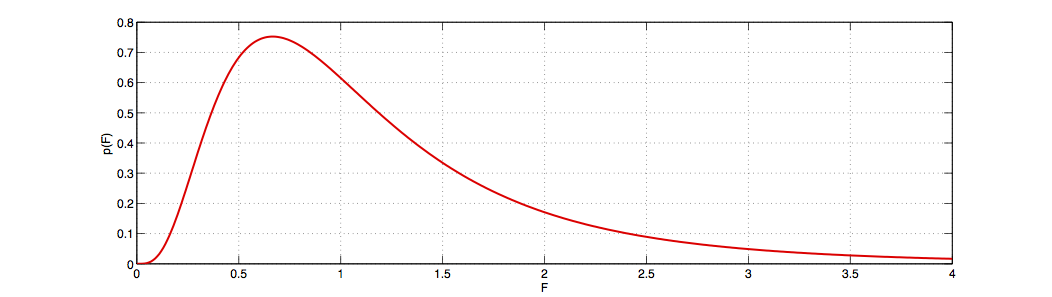
\includegraphics[width=0.85\textwidth]{fish.png}
    \end{center}
     }

     \only<2>{
     \textbf{Пример:} для веса ребёнка при рождении имеется следующая модель:
     $$weight = \beta_0 + \beta_1cigs + \beta_2parity + \beta_3inc + \beta_4med + \beta_5fed + \varepsilon,$$
     где $cigs$~---  среднее число сигарет, выкуривавшихся матерью за один день беременности, $parity$~---  номер ребёнка у матери, $inc$~--- среднемесячный доход семьи, $med$~--- длительность в годах получения образования матерью, $fed$~---  отцом.
     Данные имеются для 1191 детей.

     Зависит ли вес ребёнка при рождении от уровня образования родителей?

    \bigskip

    $H_0\colon \beta_4=\beta_5 = 0.$

    $H_1\colon H_0$ неверна $\Rightarrow p = 0.2421$.
     }
\end{frame}

\begin{frame}{Связь между критериями Фишера и Стьюдента}
%%%%%%%%%%%%%%%%%%%%%%%%%%%%%%%%%%%%%%%%%%%%%%%%%%%%%%%%%%%%%%%%%%%%%%%
% Если k1 = 1, то критерий Фишера даёт абсолютно такой же достигаемый уровень значимости, какой дал бы критерий Стьюдента для этого же самого признака при использовании двусторонней альтернативы.
% Если k1 > 1, могут возникать разные неоднозначные ситуации. Например, критерий Фишера может говорить, что гипотеза незначимости признаков X2 отвергается. При этом критерий Стьюдента не может от- вергнуть никакую из гипотез о признаках, лежащих внутри X2. Получается странная ситуация: все вместе признаки значимо определяют отклик, но отдельно ни один из них значимо на отклик не влияет. Это можно объяснить двумя способами. Во-первых, такая ситуация может возникать, если отдельные признаки из X2 недостаточно хорошо объясняют отклик, но их совокупный эффект при прогнозировании y значим. Во-вторых, признаки из X2 могут быть мультиколлинеарны. Мультиколлинеарность приводит к численной неустойчивости критериев Стьюдента и Фишера, поэтому их достигаемые уровни значимости могут быть неадекватными.
% Теперь противоположная ситуация. Пусть критерий Фишера не отвергает гипотезу о незначимости признаков из X2, а критерий Стьюдента по отдельным компонентам X2 какие-то из гипотез отвергает. То есть все вместе признаки незначимы, а какие-то из них по отдельности оказываются значимыми. Для этого тоже может быть два объяснения. Первый вариант: незначимые признаки из X2 маскируют влияние значимых. Второй вариант: значимость отдельных признаков из X2 — это результат эффекта множественной проверки гипотез. Действительно, критерии Фишера проверяют всего одну гипотезу, а критерии Стьюдента проверяют целую серию из k1 гипотез, и какие-то из них могут отклониться просто случайно.
%%%%%%%%%%%%%%%%%%%%%%%%%%%%%%%%%%%%%%%%%%%%%%%%%%%%%%%%%%%%%%%%%%%%%%%
    Если $k_1=1$, критерий Фишера эквивалентен критерию Стьюдента для двусторонней альтернативы.

    \bigskip

    Иногда критерий Фишера отвергает гипотезу о незначимости признаков $X_2$, а критерий Стьюдента не признаёт значимым ни один из них. Возможные объяснения:
    \begin{itemize}
    \item отдельные признаки из $X_2$ недостаточно хорошо объясняют $y$, но~совокупный эффект значим;
    \item признаки в $X_2$ мультиколлинеарны.
    \end{itemize}

    \bigskip

    Иногда критерия Фишера не отвергает гипотезу о незначимости признаков $X_2$, а критерий Стьюдента признаёт значимыми некоторые из них. Возможные объяснения:
    \begin{itemize}
    \item незначимые признаки в $X_2$ маскируют влияние значимых;
    \item значимость отдельных признаков в $X_2$~--- результат множественной проверки гипотез.
    \end{itemize}
\end{frame}

\begin{frame}{Критерий Фишера}
%%%%%%%%%%%%%%%%%%%%%%%%%%%%%%%%%%%%%%%%%%%%%%%%%%%%%%%%%%%%%%%%%%%%%%%
% Критерий Фишера имеет особенный вид, если требуется проверить гипотезу о том, что все признаки X для предсказания y не нужны, то есть лучшее предсказание для y — это константа.	Нулевое распределение статистики точно такое же, как и раньше, — это распределение Фишера
%%%%%%%%%%%%%%%%%%%%%%%%%%%%%%%%%%%%%%%%%%%%%%%%%%%%%%%%%%%%%%%%%%%%%%%
    \only<1>{
    \begin{center}
        \begin{tabular}{rl}
            нулевая гипотеза:               & $H_0\colon \beta_1 = \dots = \beta_k=0$ \\
            альтернатива:                   & $H_1\colon H_0$ неверна\\
            статистика:                     & $F = \frac{R^2 / k}{\left(1-R^2\right) / \left(n-k-1\right)}$ \\
            нулевое распределение:          & $F(k,n-k-1)$\\
        \end{tabular}
        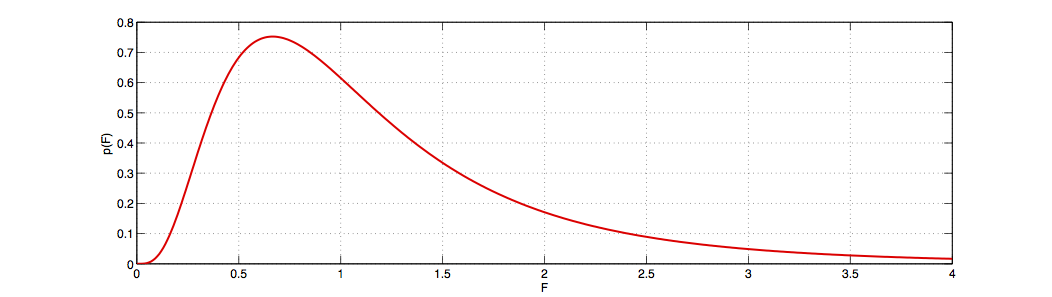
\includegraphics[width=0.85\textwidth]{fish.png}
    \end{center}
     }

     \only<2>{
     \textbf{Пример:} имеет ли вообще смысл модель веса ребёнка при рождении, рассмотренная выше?

    \bigskip

    $H_0\colon \beta_1=\dots=\beta_5 = 0.$

    $H_1\colon H_0$ неверна $\Rightarrow p = 6.0331\times10^{-9}$.
     }
\end{frame}

\begin{frame}{Сравнение невложенных моделей}
    \textbf{Пример}: имеются две модели:
    \begin{align}
    y &= \beta_0 + \beta_1x_1 + \beta_2x_2+\varepsilon, \label{m1} \\
    y &= \gamma_0 + \gamma_1\log x_1 + \gamma_2\log x_2+\varepsilon. \label{m2}
    \end{align}

    \bigskip

    Как понять, какая из них лучше?
\end{frame}

\begin{frame}{Критерий Давидсона-Маккиннона}
    Пусть $\hat{y}$~--- оценка отклика по первой модели, $\hat{\hat{y}}$~--- по второй.

    Подставим эти оценки как признаки в чужие модели:
    \begin{align*}
    y &= \beta_0 + \beta_1x_1 + \beta_2x_2+\beta_3\hat{\hat{y}}+\varepsilon, \\
    y &= \gamma_0 + \gamma_1\log x_1 + \gamma_2\log x_2+\gamma_3\hat{y}+\varepsilon.
    \end{align*}

    \bigskip

    При помощи критерия Стьюдента проверим
    \begin{align*}
    H_{01}\colon \beta_3=0,\; & \;H_{11}\colon \beta_3\neq0, \\
    H_{02}\colon \gamma_3=0,\; & \;H_{12}\colon \gamma_3\neq0.
    \end{align*}

    \bigskip

    \begin{center}
    \begin{tabular}{|c|p{9em}|p{9em}|}
        \hline
        \diagbox{$H_{01}$}{$H_{02}$} & Принята                         & Отвергнута   \\                   \hline
        Принята                           & Обе модели хороши               & Модель \eqref{m1} значимо лучше \\\hline
        Отвергнута                        & Модель \eqref{m2} значимо лучше & Обе модели плохи  \\        \hline
    \end{tabular}
    \end{center}
\end{frame}

\subsection{Отбор признаков}
\begin{frame}{Пошаговая регрессия}
    \begin{itemize}
    \item \textbf{Шаг 0}. Настраивается модель с одной только константой, а также все модели с одной переменной.
          Рассчитывается $F$-статистика каждой модели и достигаемый уровень значимости.
          Выбирается модель с~наименьшим достигаемым уровнем значимости.
          Соответствующая переменная $X_{e1}$ включается в модель, если этот достигаемый уровень значимости меньше порогового значения $p_E = 0.05$.
    \item \textbf{Шаг 1}. Рассчитывается $F$-статистика и достигаемый уровень значимости для всех моделей, содержащих две переменные, одна из которых $X_{e1}$.
          Аналогично принимается решение о включении $X_{e2}$.
    \item \textbf{Шаг 2}. Если была добавлена переменная $X_{e2}$, возможно, $X_{e1}$ уже не~нужна.
          В общем случае просчитываются все возможные варианты исключения одной переменной, рассматривается вариант с~наибольшим достигаемым уровнем значимости, соответствующая переменная исключается, если он превосходит пороговое значение $p_R = 0.1$.
    \item \dots
    \end{itemize}
\end{frame}

\begin{frame}{Эксперимент Фридмана}
    Сгенерируем полноранговую матрицу $\mathbf{X}$ размера $n\times m$ и вектор $\mathbf{y}$.\\
    При $n \to \infty, \frac{n}{m} \to \rho$: $R^2 \to \rho.$  \bigskip
    
    (Freedman, 1983): пошаговая регрессия несовместима с проверкой гипотез о значимости коэффициентов: критерии Фишера и Стьюдента антиконсервативны, если вычисляются на той же самой выборке, на~которой настраивалась модель.
\end{frame}

\begin{frame}{Отбор признаков с учётом эффекта множественной проверки гипотез}
    $\forall c_1,\dots,c_{k_1} \in \mathbb{R}^{k+1}$
    $$t_j = \frac{c_j^T \left(\beta-\hat{\beta}\right)}{\hat{\sigma} \sqrt{c_j^T \left(X^TX\right)^{-1}c_j}}, \;\; j=1,\dots,k_1$$
    имеют совместное распределение Стьюдента с числом степеней свободы $n-k-1$ и корреляционной матрицей
    \begin{align*}
    R &= DC^T \left(X^TX\right)^{-1} CD,\\
    C &= \left(c_1,\dots,c_{k_1}\right), \\
    D &= \diag\left(c_j^T \left(X^TX\right)^{-1}c_j\right)^{-\frac1{2}}.
    \end{align*}

    \bigskip

    Для одновременной проверки значимости всех коэффициентов регрессии достаточно взять в качестве $C$ единичную матрицу.
\end{frame}


\begin{frame}{Значимость категориальных предикторов}	
	Категориальный предиктор, кодируемый несколькими фиктивными переменными, необходимо включать или исключать целиком. Значимость соответствующих фиктивных переменных лучше проверять в совокупности.
	
	\bigskip
	
	В случае, когда по отдельности какие-то фиктивные переменные не~значимы, допустимо объединять уровни категориального предиктора, основываясь на интерпретации.
\end{frame}

\subsection{Анализ остатков}


\begin{frame}{Проверка предположений Гаусса-Маркова}
%%%%%%%%%%%%%%%%%%%%%%%%%%%%%%%%%%%%%%%%%%%%%%%%%%%%%%%%%%%%%%%%%%%%%%%
% Первое предположение — это предположение о линейности отклика. Утверждается, что y в действительности представляет собой линейную комбинацию X с какой-то случайной ошибкой. Естественно, это предположение в точности не выполняется никогда. Трудно ожидать, что отклик y в действи- тельности — это линейная комбинация рассматриваемых признаков x. Линейная модель, как и все остальные, неверна, но очень полезна, и кроме того, устойчива к небольшим отклонениям от линейности. Поэтому единственное, что требуется проверить, — это нет ли каких-то огромных отклонений от линейности y по x. Чтобы убедиться в отсутствии больших отклонений от линейнойсти, нужно анализировать остатки. Для остатков необходимо построить графики. По горизонтальной оси откладывается значение каждого из признаков xj , по вертикальной оси — остатки, и нужно смотреть, как выглядит получающееся облако точек. Если, например, оно выглядит как на рисунке 10.4, представляет собой какую-то параболу, то, скорее всего это значит, что отклик y зависит от квадрата признака xj . Такую зависимость можно учесть, просто добавив в матрицу X столбец, соответствующий x2j . На таком графике можно обнаруживать и другие осмысленные функциональные зависимости. Если такие зависимости видны, нужно просто добавить в матрицу X соответствующий столбец.
% Следующее предположение — это предположение о случайности выборки. Требуется, чтобы выборка была независимой и одинаково распределенной. Это предположение может нарушаться несколькими способами. Первый способ более тяжелый: если объекты, на которых измерены признаки и отклик, зависимы, то всё плохо: дисперсии ошибки и коэффициентов недооцениваются, и все статистические критерии, которые на этом основаны, перестают работать корректно. Еще это предположение может нарушаться, если выборка отобрана из генеральной совокупности не слу- чайно, а каким-то образом отфильтрована. Фильтровать генеральную совокупность по какому-то признаку z можно только в случае, если E(y|x,z) = E(y|x), то есть z не добавляет никакой новой информации об y. Если выборка отфильтровывалась как-то иначе, например, просто по одному из признаков, содержащихся в x, то выводы, построенные по такой модели, можно распространять только на отфильтрованную генеральную совокупность. Например, если в выборке испытуемые только младше 50 лет, то нельзя ничего сказать об испытуемых в генеральной совокупности, которым больше 50 лет.
% Следующее предположение: матрица X должна иметь полный столбцовый ранг. Если в выборке есть линейно зависимые признаки, то дисперсия оценки коэффициентов при таких призна- ках будет бесконечной. Это не очень удобно при построении доверительных интервалов: они будут иметь бесконечную ширину. И кроме того, гипотезы тоже так не проверить. Если возникла такая проблема, это значит, что от каких-то признаков в модели придется избавиться. Помимо всего прочего, для категориальных переменных нельзя использовать one-hot encoding. Дело в том, что при кодировании каждого уровня фактора своей бинарной переменной мы получаем, что в сумме такие переменные дают единичный столбец, а он в матрице X уже есть, поэтому столбцы получаются линейно зависимы. Вместо этого нужно использовать dummy-кодирование.
%%%%%%%%%%%%%%%%%%%%%%%%%%%%%%%%%%%%%%%%%%%%%%%%%%%%%%%%%%%%%%%%%%%%%%%
    \begin{enumerate}
    \item Линейность отклика: $y = X\beta+\varepsilon.$
    \item Случайность выборки: наблюдения $(x_i,y_i), i=1,\dots,n$ независимы.
    \begin{itemize}
    \item Предположения (1-2) проверить нельзя.
    \end{itemize}
    \item Полнота ранга: ни один из признаков не является константой или линейной комбинацией других признаков ни в популяции, ни в~выборке ($\rank X = k+1$).
    \begin{itemize}
    \item Предположение (3) легко проверяется, без его выполнения построить модель вообще невозможно.
    \end{itemize}
     \item Случайность ошибок: $\mathbb{E}\left(\varepsilon\left|X\right.\right) = 0.$
     \item Гомоскедастичность ошибок: дисперсия ошибки не зависит от~значений признаков: $\mathbb{D}\left(\varepsilon\left|X\right.\right)=\sigma^2.$
    \item Нормальность ошибок: $\varepsilon\left| X\right. \sim N\left(0,\sigma^2\right).$
    \begin{itemize}

    \item Предположения (4-6) об ошибке $\varepsilon$ необходимо проверять.
    \end{itemize}
    \end{enumerate}

    \bigskip

    Оценивать ошибку $\varepsilon$ будем при помощи \textbf{остатков}:
    $$\hat{\varepsilon}_i = y_i - \hat{y}_i, \; i=1,\dots,n.$$
    Стандартизированные остатки:
    $$\tilde{\varepsilon}_i = \frac{\hat{\varepsilon}_i}{\hat{\sigma}}, \; i=1,\dots,n.$$
\end{frame}

\begin{frame}{Визуальный анализ}
    \only<1>{
    Строятся графики зависимости $\tilde{\varepsilon}_i$ от $\hat{y}_i$, \; $x_{ij}, j=1,\dots,k,$ \; $i$.
    \begin{center}
            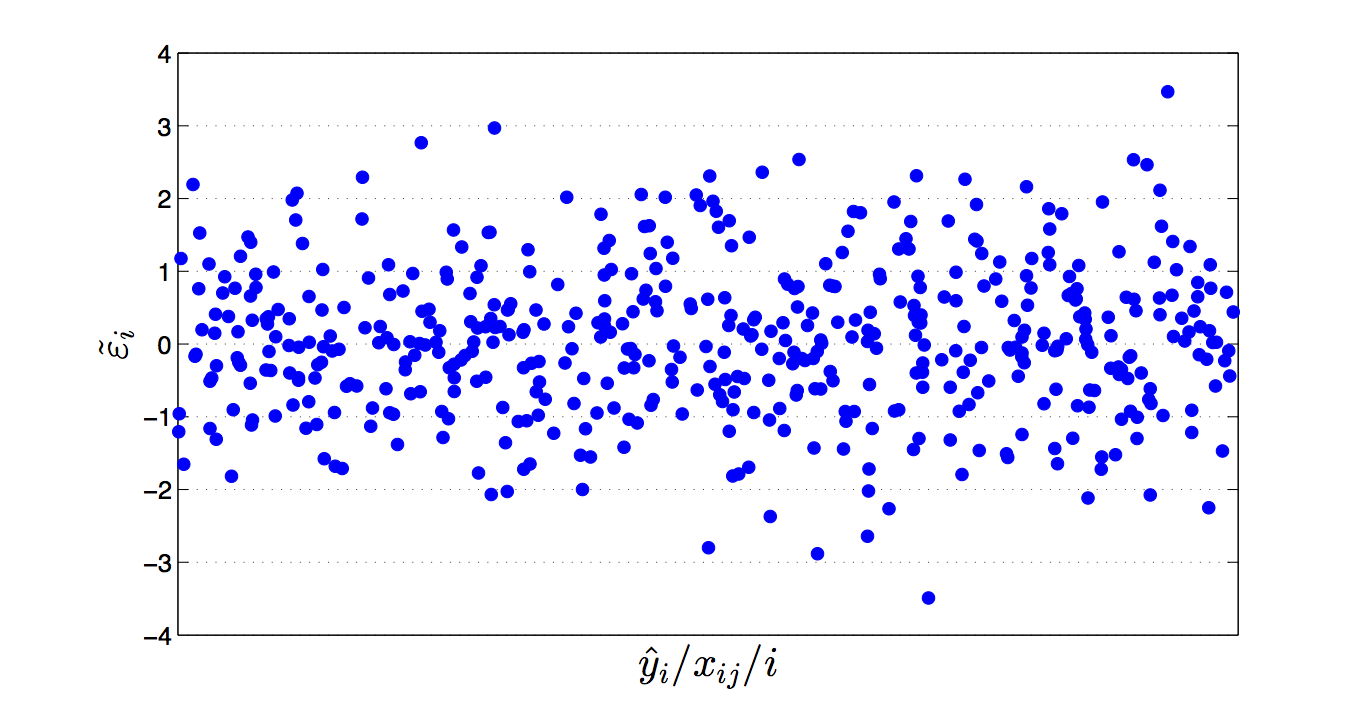
\includegraphics[width=0.85\textwidth]{goodres.png}
    \end{center}
    }

    \only<2>{
    \begin{center}
            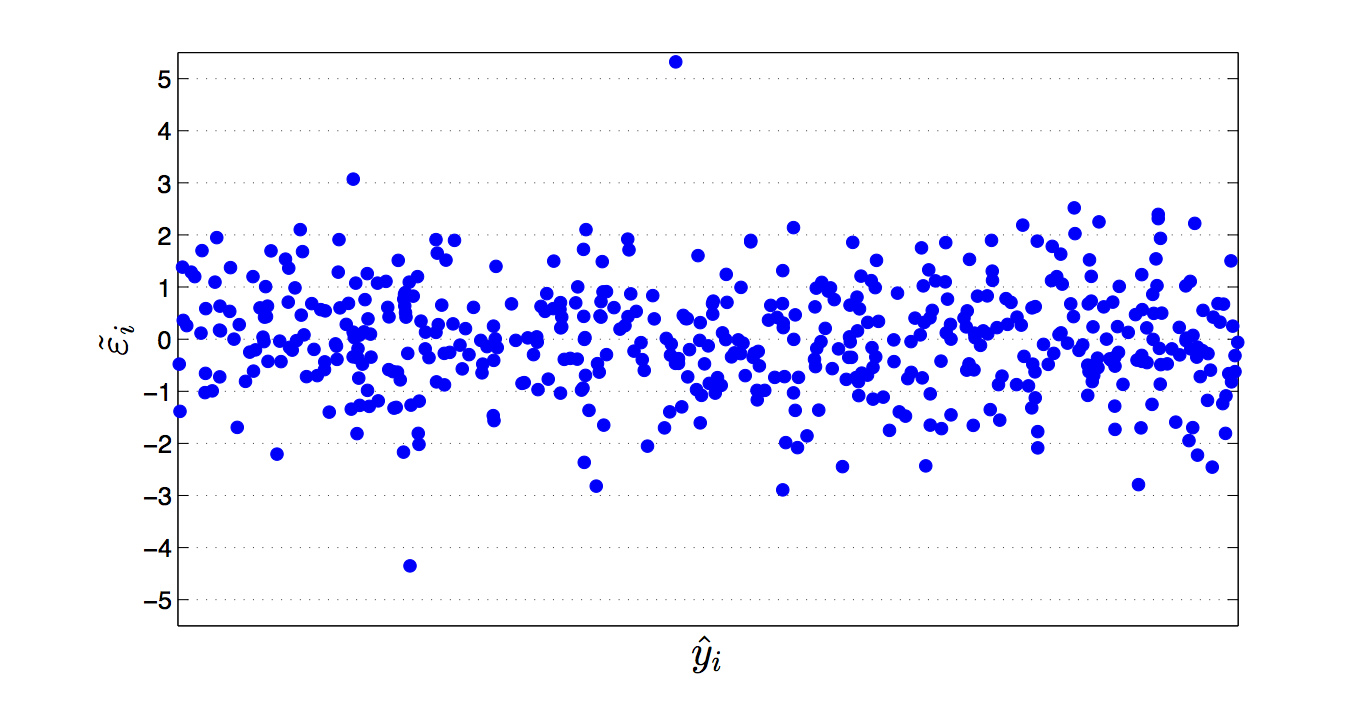
\includegraphics[width=0.85\textwidth]{outres.png}
    \end{center}

    \bigskip

    Возможно, присутствуют выбросы
    }

    \only<3>{
    \begin{center}
            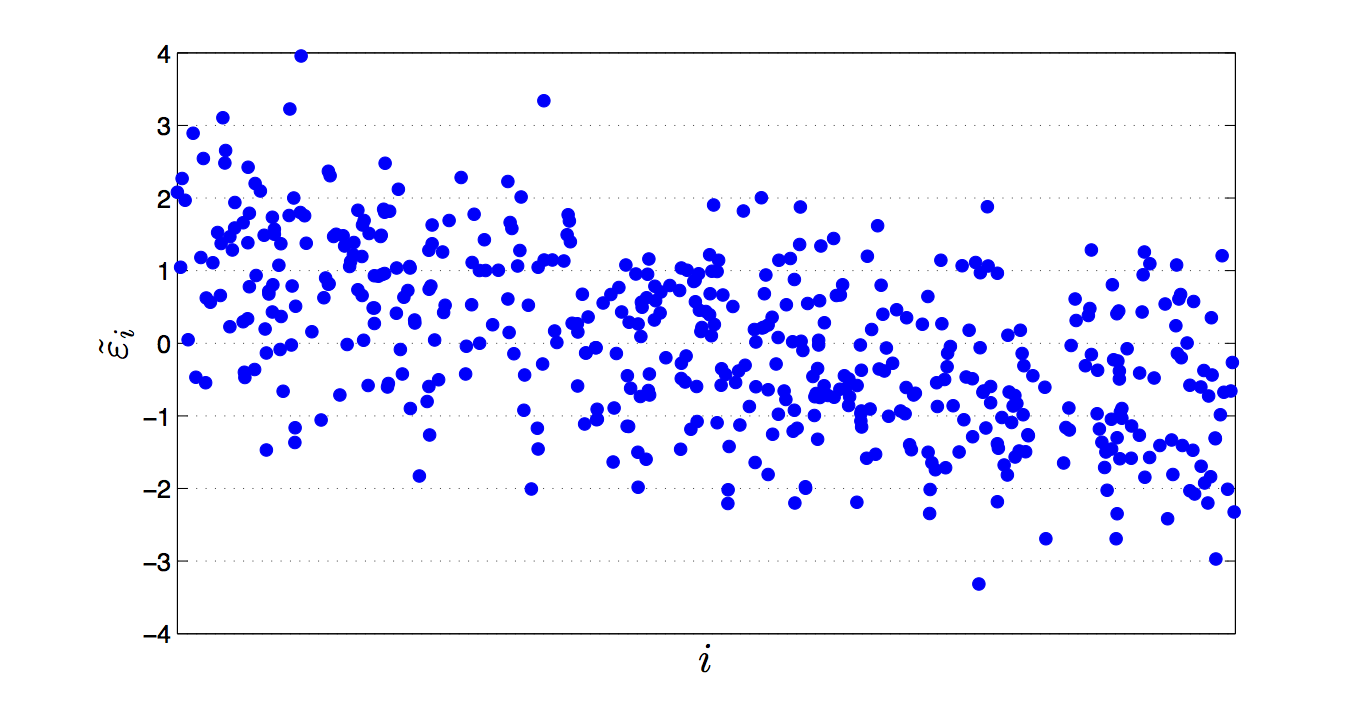
\includegraphics[width=0.85\textwidth]{trendres.png}
    \end{center}

    \bigskip

    В данных имеется тренд
    }

    \only<4>{
    \begin{center}
            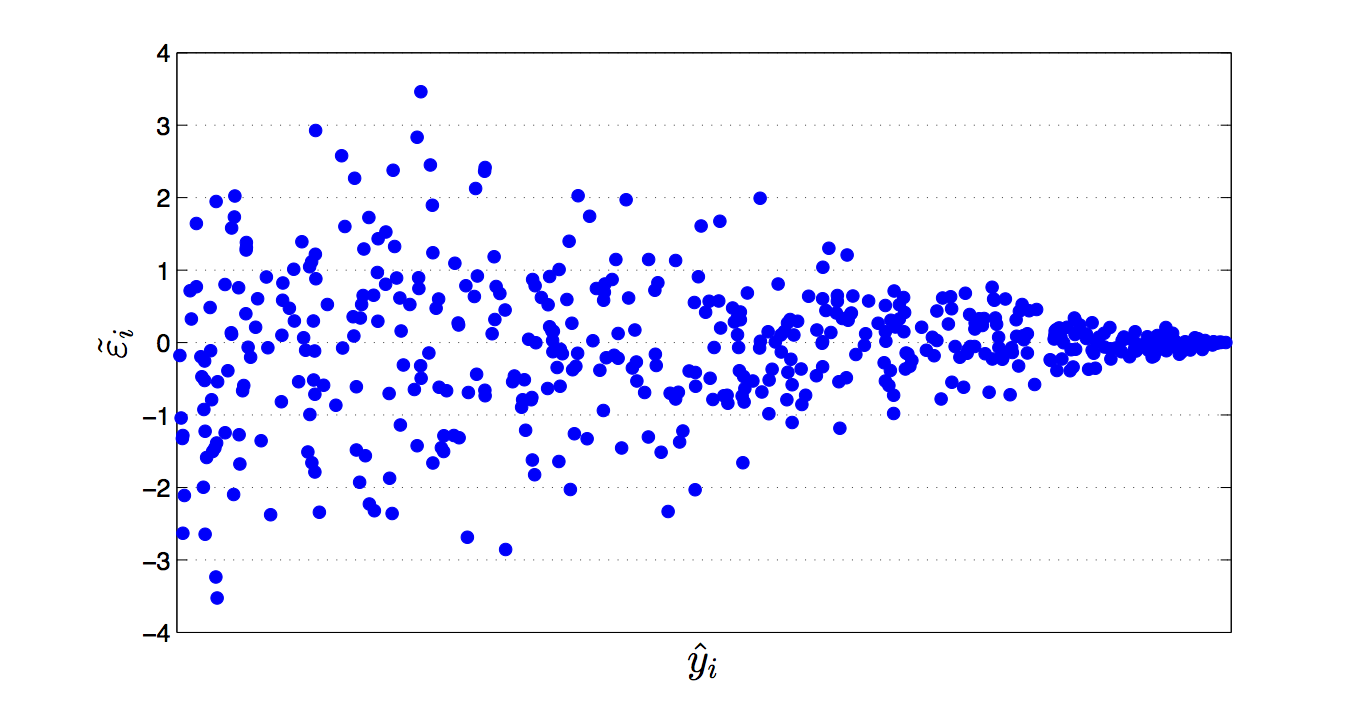
\includegraphics[width=0.85\textwidth]{heterores.png}
    \end{center}

    \bigskip

    Гетероскедастичность
    }

    \only<5>{
    \begin{center}
            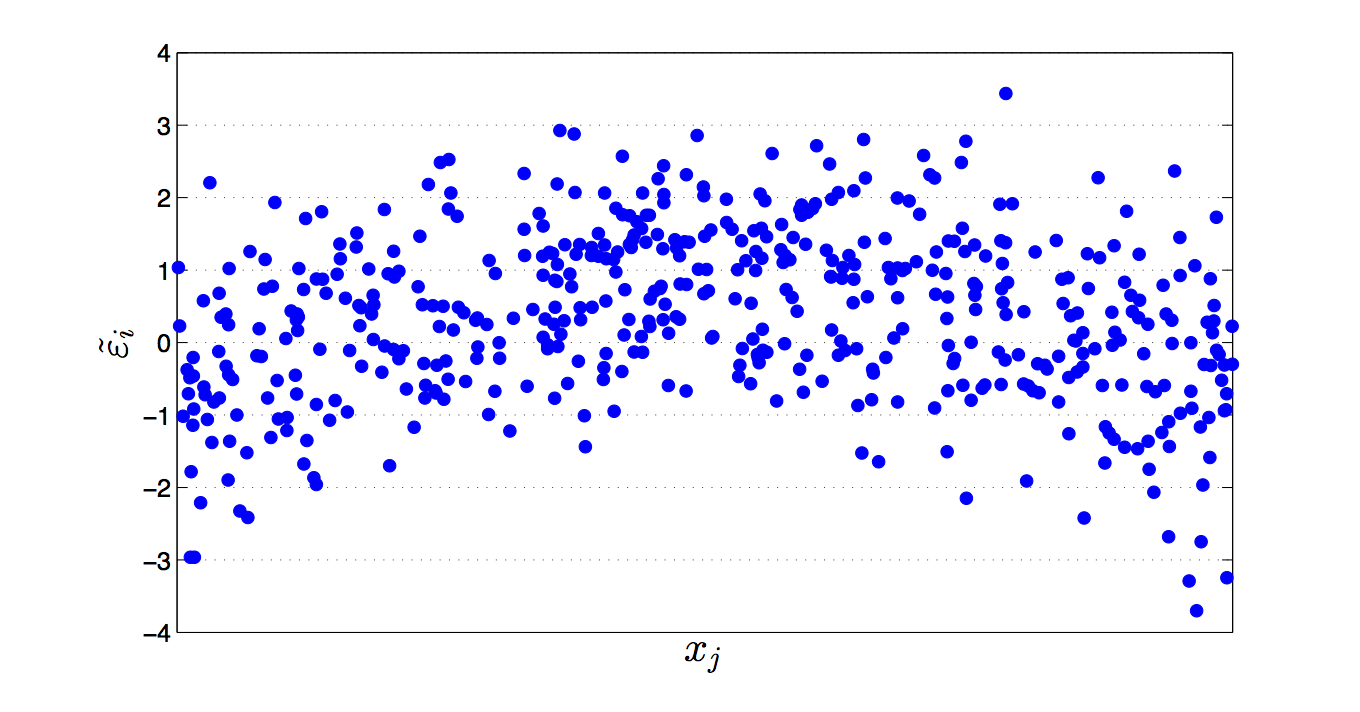
\includegraphics[width=0.85\textwidth]{squaredres.png}
    \end{center}

    \bigskip

    Стоит добавить квадрат признака $x_j$
    }
\end{frame}

\begin{frame}{Формальные критерии}
%%%%%%%%%%%%%%%%%%%%%%%%%%%%%%%%%%%%%%%%%%%%%%%%%%%%%%%%%%%%%%%%%%%%%%%
% Способы проверки нормальности уже разбирались ранее. Есть визуальный способ: нужно построить ку-ку график и посмотреть, лежат ли точки на этом графике более-менее на одной прямой. Также есть формальный способ: можно использовать статистиче- ские критерии для проверки нормальности. Среди всего разнообразия критериев рекомендуется использовать критерий Шапиро-Уилка.
% Гипотезу о случайности ошибки можно очень легко проверить по данным. Для этого нужно построить регрессию y по x, вычислить остатки и проверить гипотезу о том, что среднее значение остатков равно 0. Это можно сделать, например, с помощью критерия Стьюдента.
% предположение гомоскедастичности ошибки можно проверять двумя способами. Первый, нестрогий, — это визуальный анализ. Нужно построить графики зависимости остатков от всех признаков xj и посмотреть, выглядят ли точки на этом графике как горизонтальная полоса. Если вместо горизонтальной полосы на графике изображено что-то расширяющееся или сужающееся, значит, предположение гомоскедастичности не выполняется. Формально это предположение можно проверять с помощью критерия Бройша-Пагана
%%%%%%%%%%%%%%%%%%%%%%%%%%%%%%%%%%%%%%%%%%%%%%%%%%%%%%%%%%%%%%%%%%%%%%%
    \begin{itemize}
    \item Проверка нормальности --- занятие~2.
    \item Проверка несмещённости: если остатки нормальны~--- критерий Стьюдента (занятие 2), нет~--- непараметрический критерий (занятие~3).
    \item Проверка гомоскедастичности: критерий Бройша-Пагана.
    \end{itemize}
\end{frame}

\begin{frame}{Критерий Бройша-Пагана}
    \begin{center}
        \begin{tabular}{rl}
            нулевая гипотеза:               & $H_0\colon \mathbb{D}\varepsilon_i = \sigma^2$ \\
            альтернатива:                   & $H_1\colon H_0$ неверна\\
            статистика:                     & $LM = n R^2_{\hat{\varepsilon}^2}, \; R^2_{\hat{\varepsilon}^2}$~--- коэффициент детерминации \\
                                            & при регрессии квадратов остатков на признаки \\
            нулевое распределение:          & $\chi^2_{k}$\\
        \end{tabular}
        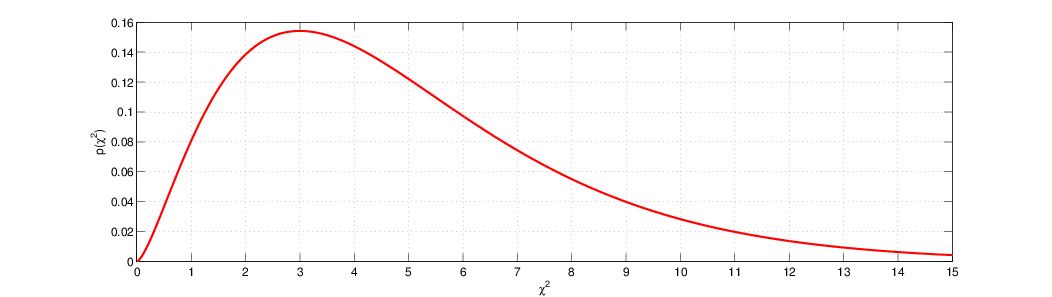
\includegraphics[width=0.85\textwidth]{chi2.png}
    \end{center}
\end{frame}

\subsection{Гетероскедастичность}
\begin{frame}{Гетероскедастичность}
    Гетероскедастичность может быть следствием недоопределения модели.

    \bigskip

    Последствия гетероскедастичности:
    \begin{itemize}
    \item МНК-оценки $\beta$ и $R^2$ остаются несмещёнными и состоятельными
    \item нарушаются предположения критериев Стьюдента и~Фишера и~методов построения доверительных интервалов для $\sigma$ и $\beta$ (независимо от объёма выборки) %оценки дисперсии смещены, нарушаются предположения основанных на них методов анализа моделей (дальше) 
    \end{itemize}

    \bigskip

    Варианты:
    \begin{itemize}
    \item переопределить модель, добавить признаки, преобразовать отклик
    \item использовать модифицированные оценки дисперсии коэффициентов
    \end{itemize}
\end{frame}

\begin{frame}{Преобразование Бокса-Кокса}
    Пусть значения отклика $y_1,\dots,y_n$ положительны. Если $\frac{\max y_i}{\min y_i}>10,$ стоит рассмотреть возможность преобразования $y$. В каком виде его искать?

    \bigskip

    Часто полезно рассмотреть преобразования вида $y^\lambda$, но оно не имеет смысла при $\lambda=0.$

    Вместо него можно рассмотреть семейство преобразований
    $$W=\begin{cases}
            \left(y^\lambda-1\right)/\lambda, & \lambda\neq 0, \\
            \ln y, & \lambda=0.
        \end{cases}
    $$
    но оно сильно варьируется по $\lambda$.

    Вместо него можно рассмотреть семейство преобразований
    $$V=\begin{cases}
            \left(y^\lambda-1\right)/\left(\lambda \dot{y}^{\lambda-1}\right), & \lambda\neq 0, \\
            \dot{y}\ln y, & \lambda=0,
        \end{cases}
    $$
    где $\dot{y} = \left(y_1y_2\dots y_n\right)^{1/n}$~--- среднее геометрическое наблюдений отклика.
\end{frame}

\begin{frame}{Метод Бокса-Кокса}
    Процесс подбора $\lambda$:
    \begin{enumerate}
    \item выбирается набор значений $\lambda$ в некотором интервале, например, $\left(-2,2\right)$;
    \item для каждого значения $\lambda$ выполняется преобразование отклика $V$, строится регрессия $V$ на $X$, вычисляется остаточная сумма квадратов $RSS(\lambda);$
    \item строится график зависимости $RSS(\lambda)$ от $\lambda$, по нему выбирается оптимальное значение $\lambda$;
    \item выбирается ближайшее к оптимальному удобное значение $\lambda$ (например, целое или полуцелое);
    \item строится окончательная регрессионная модель с откликом $y^\lambda$ или $\ln y$.
    \end{enumerate}

    \bigskip

    Доверительный интервал для $\lambda$ определяется как пересечение кривой $RSS\left(\lambda\right)$ с линией уровня $\min\limits_{\lambda} RSS\left(\lambda\right) \cdot e^{\chi_{1, 1-\alpha}^2/n}.$
    Если он содержит единицу, возможно, не стоит выполнять преобразование.
\end{frame}

\begin{frame}{Устойчивая оценка дисперсии Уайта}
    Если не удаётся избавиться от гетероскедастичности, при анализе моделей (дальше) можно использовать устойчивые оценки дисперсии.

    White's heteroscedasticity-consistent estimator (HCE):
    $$\mathbb{D}\left(\left.\hat{\beta}\right|X\right) = \left(X^TX\right)^{-1} \left(X^T \diag \left(\hat{\varepsilon}^2_1, \dots, \hat{\varepsilon}^2_n\right) X\right) \left(X^TX\right)^{-1}.$$
    
    \bigskip

    Асимптотика устойчивой оценки:
    $$\sqrt{n} \left(\beta - \hat{\beta}\right) \xrightarrow{d} N\left(0, \Omega\right),$$
    $$\hat{\Omega} = n \left(X^TX\right)^{-1} \left(X^T \diag \left(\hat{\varepsilon}^2_1, \dots, \hat{\varepsilon}^2_n\right) X\right) \left(X^TX\right)^{-1}.$$    
\end{frame}

\begin{frame}{Другие устойчивые оценки дисперсии}
    Элементы диагональной матрицы могут задаваться разными способами:

    \bigskip

    \begin{center}
    \begin{tabular}{c c}
      const & $\hat{\sigma}^2$ \\
      HC0   & $\hat{\varepsilon}^2_i$  \\
      HC1   & $\frac{n}{n-k}\hat{\varepsilon}^2_i$  \\
      HC2   & $\frac{\hat{\varepsilon}^2_i}{1-h_i}$  \\
      HC3   & $\frac{\hat{\varepsilon}^2_i}{\left(1-h_i\right)^2}$  \\
      HC4   & $\frac{\hat{\varepsilon}^2_i}{\left(1-h_i\right)^{\min\left(4, \frac{nh_i}{k}\right)}}$  \\
    \end{tabular}
    \end{center}

    \bigskip

    const --- случай гомоскедастичной ошибки,

    HC0 --- оценка Уайта,

    HC1--HC3 --- модификации МакКиннона-Уайта,

    HC4 --- модификация Крибари-Нето.
\end{frame}


\subsection{Выбросы}
\begin{frame}{Расстояние Кука}
	\only<1>{	
		Регрессия сильно подстраивается под далеко стоящие наблюдения.
		
		\begin{center}
			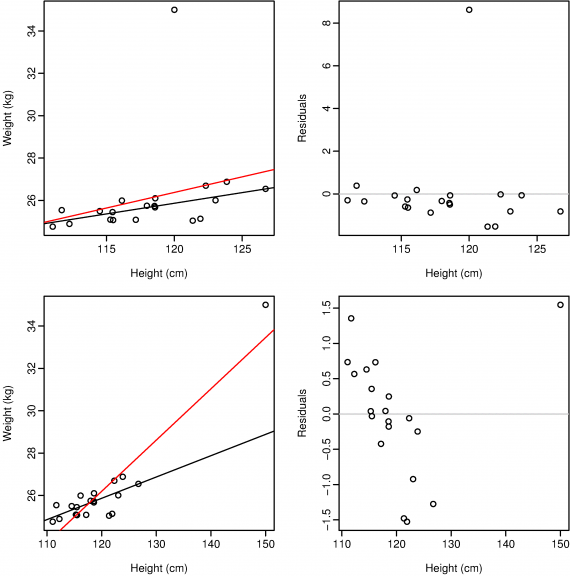
\includegraphics[height=0.8\textheight]{leverage.png}
		\end{center}	
	}
	
	\only<2>{	
	
	Расстояние Кука --- мера воздействия $i$-го наблюдения на регрессионное уравнение:
	$$D_i = \frac{\sum\limits_{j=1}^n \left(\hat{y}_j - \hat{y}_{j(i)}\right)^2}{RSS\left(k+1\right)} = \frac{\hat{\varepsilon}_i^2}{RSS\left(k+1\right)} \frac{h_{i}}{\left(1-h_{i}\right)^2},$$
	$\hat{y}_{j(i)}$~--- предсказания модели, настроенной по наблюдениям $1,\dots,i-1,i+1,\dots,n,$ для наблюдения $j;$
	
	$h_{i}$ --- диагональный элемент матрицы $H=X\left(X^TX\right)^{-1}X^T$ (hat matrix).
	
	\bigskip
	
	Варианты порога на $D_i$:
	\begin{itemize}
		\item $D_i=1$;
		\item $D_i=4/n$;
		\item $D_i = 3\bar{D}$;
		\item визуально по графику зависимости $D_i$ от $\hat{y}_i$.
	\end{itemize}
}
\end{frame}

%\section{Итог}
%\subsection{Пример}
%\begin{frame}{Пример}
%	Привлекательность и уровень заработной платы: 
%	
%	\url{https://yadi.sk/d/Lf2g2bMGfDM2N}
%\end{frame}

\section{}
\begin{frame}{Литература}
    \only<1>{
    \begin{itemize}
    \item линейная регрессия в целом~--- Wooldridge (много примеров, без матричной алгебры);
    \item критерий Давидсона-Маккиннона (Davidson-MacKinnon test)~--- Davidson;
    \item множественная оценка значимости коэффициентов~--- Bretz, 4.4;
    \item преобразование Бокса-Кокса (Box-Cox transformation)~--- Дрейпер, гл.~14;        
    \item устойчивые оценки дисперсии~--- White, MacKinnon, Cribari-Neto;
    \item расстояние Кука (Cook's distance)~--- Cook. %;
%    \item доверительные ленты~--- Liu.
    \end{itemize}
    
    \bigskip
    
    {\small 
    Дрейпер Н.Р., Смит Г. \textit{Прикладной регрессионный анализ}, 2007.
    
    \vspace{5pt}    		
    
    Кобзарь А.И. \textit{Прикладная математическая статистика}, 2006.
    
    \vspace{5pt}    		
    
    Bretz F., Hothorn T., Westfall P. \textit{Multiple Comparisons Using R}, 2010.   	
    		
    \vspace{5pt}    		
    		
     Cook D.R., Weisberg S. \textit{Residuals and influence in regression}, 1982.
   }
  }
  
  \only<2>{
  	{\small  
  	Avenhaus R. et al. 1980 \textit{Approaches to Inverse Linear Regression}		
    Cribari-Neto F. (2004). \textit{Asymptotic inference under heteroskedasticity of unknown form}. Computational Statistics \& Data Analysis, 45(2), 215–233.
    		
    		\vspace{5pt}    		
    		
    Davidson R., MacKinnon J. (1981). \textit{Several Tests for Model Specification in the Presence of Alternative Hypotheses}. Econometrica, 49, 781-793.
    		
    		\vspace{5pt}    		
    		
    Freedman D.A. \textit{A Note on Screening Regression Equations}. The American Statistician, 37(2), 152-155.
    		
    		\vspace{5pt}    	
    		    		
%    Liu W. \textit{Simultaneous Inference in Regression}, 2010.
%    		
%    		\vspace{5pt}    		
%    		
    MacKinnon J., White H. (1985). \textit{Some heteroskedasticity-consistent covariance matrix estimators with improved finite sample properties}. Journal of Econometrics, 29, 305–325.
    		
    		\vspace{5pt}    		
    		
    White H. (1980). \textit{A heteroskedasticity-consistent covariance matrix estimator and a~direct test for heteroskedasticity}. Econometrica: Journal of the Econometric Society, 48(4), 817–838.
    		
    		\vspace{5pt}    		
    		
    Wooldridge J. \textit{Introductory Econometrics: A Modern Approach}, 2016.
    }
    }
\end{frame}

\end{document}
